\documentclass[11pt,aspectratio=169]{beamer}
\usepackage[portuguese]{babel}
\usepackage{graphicx,booktabs,amsmath,amssymb}
\usepackage{appendixnumberbeamer}   % slides de reserva nao entram na contagem
\usepackage{tikz}
\usetikzlibrary{positioning,arrows.meta}
\graphicspath{{figuras/}}
\usetheme{Madrid}                   % cores padrao do Madrid, derivadas automaticamente

% ajustes minimos
\setbeamertemplate{navigation symbols}{}
\setbeamertemplate{itemize items}[circle]
\setbeamercolor{alerted text}{use=structure, fg=structure.fg}  % destaque no azul do tema, em negrito
\setbeamerfont{alerted text}{series=\bfseries}

% sumario automatico no inicio de cada secao, com a secao atual em destaque
\AtBeginSection[]{%
  \begin{frame}{Roteiro}
    \tableofcontents[currentsection]
  \end{frame}}

% legenda curta abaixo das figuras e botoes da reserva
\newcommand{\fonte}[1]{\par\vspace{2pt}{\scriptsize\color{black!65}#1\par}}
\newcommand{\reserva}[2]{\hyperlink{#1}{\beamergotobutton{#2}}}
\newcommand{\voltar}[2]{\hyperlink{#1}{\beamerreturnbutton{#2}}}
\newcommand{\indicereserva}{\hfill\hyperlink{reservas}{\beamerskipbutton{Índice da reserva}}}

\title[Canal de crédito e política monetária no Brasil]{O canal de crédito na transmissão da política monetária no Brasil}
\subtitle{Evidências de um modelo VAR estrutural (2011--2025)}
\author[João Victor A. K. Santana]{João Victor Alonso Kutianski Santana}
\institute[IE -- UFRJ]{Instituto de Economia -- UFRJ\\[3pt]
  {\footnotesize Orientador: Prof. Dr. Antonio Luis Licha\\
  Coorientadora: Profa. Dra. Viviane Luporini}}
\date[Nov. 2026]{Novembro de 2026}
\titlegraphic{
\includegraphics[height=1.1cm]{logo_ufrj.png}}

\begin{document}

\begin{frame}[plain]
  \titlepage
\end{frame}

%==============================================================================
\section{Introdução}
%==============================================================================

\begin{frame}{Motivação}
  \begin{itemize}
    \item A Selic segue entre as taxas básicas \alert{mais altas do mundo}, mesmo após o Plano Real e o regime de metas
    \item Segura-Ubiergo (2012, FMI) aponta, entre as causas, a possível \alert{obstrução dos canais de transmissão}
    \item O crédito direcionado, com taxas reguladas e funding próprio, responde por \alert{42,6\% do estoque} de crédito (dez./2025)
    \item Se parte do crédito não reage à Selic, o Banco Central precisa de \alert{mais juros} para obter o mesmo efeito
  \end{itemize}
  \vspace{6pt}
  \begin{block}{Um indício}
    Leigh e Xu (2025): para elevar as taxas médias de empréstimo em 1 p.p., a Selic precisa subir cerca de 1,4 p.p.
  \end{block}
\end{frame}

\begin{frame}{Pergunta, objetivo e contribuições}
  \begin{block}{Pergunta}
    Choques na Selic afetam o \alert{custo} e o \alert{volume} do crédito livre e, por meio dele, a \alert{atividade econômica}?
  \end{block}
  \vspace{4pt}
  \textbf{Objetivo:} medir o canal de crédito no Brasil entre março de 2011 e agosto de 2025 com um VAR estrutural\\[6pt]
  \textbf{Contribuições}
  \begin{enumerate}
    \item Atualiza a evidência: recessão de 2014--2016, Selic a 2\%, pandemia e aperto desde 2021
    \item Separa \alert{preço} (spread) e \alert{quantidade} (saldo) dentro do crédito livre
    \item Testa a segmentação diretamente, com crédito livre e direcionado no mesmo modelo
  \end{enumerate}
\end{frame}

\begin{frame}{Principais resultados}
  \begin{itemize}
    \item O aperto monetário \alert{encarece o crédito livre}: o spread sobe até 0,38 p.p., do 4º ao 22º mês
    \item O \alert{volume} de crédito livre cai mais devagar e com menos intensidade: $-$0,31\% em dois anos
    \item O crédito \alert{importa para a atividade}: explica 15\% da variância do IBC-Br em dois anos, contra menos de 1\% da Selic
    \item O crédito direcionado \alert{não responde} à Selic
  \end{itemize}
  \vspace{6pt}
  \begin{block}{Conclusão}
    O canal de crédito existe no Brasil, mas a segmentação entre crédito livre e direcionado o obstrui parcialmente.
  \end{block}
\end{frame}

%==============================================================================
\section{Canal de crédito e contexto}
%==============================================================================

\begin{frame}[label=teoria]{O canal de crédito: Bernanke e Gertler (1995)}
  \setlength{\leftmargini}{1.1em}
  \begin{columns}[T]
    \begin{column}{0.32\textwidth}
      \begin{block}{O enigma}
        \footnotesize
        O custo do capital, sozinho, não explica:
        \begin{itemize}
          \item \alert{Magnitude:} efeito grande sobre gastos pouco sensíveis ao custo do capital
          \item \alert{Defasagem:} o investimento cai depois que os juros já voltaram
          \item \alert{Composição:} a habitação reage primeiro, embora dependa de juros longos
        \end{itemize}
      \end{block}
    \end{column}
    \begin{column}{0.32\textwidth}
      \begin{block}{Prêmio de financiamento externo}
        \footnotesize
        \begin{itemize}
          \item Custo de se financiar com terceiros menos o de usar recursos próprios
          \item Nasce da assimetria de informação
          \item Maior quanto menor o patrimônio do tomador
          \item O aperto eleva o juro \alert{e} o prêmio: o crédito \alert{amplifica} o canal dos juros
        \end{itemize}
      \end{block}
    \end{column}
    \begin{column}{0.32\textwidth}
      \begin{block}{Dois canais}
        \footnotesize
        \textbf{Balanço patrimonial:} juros $\uparrow$ $\Rightarrow$ colateral e patrimônio $\downarrow$ $\Rightarrow$ prêmio~$\uparrow$\\[4pt]
        \textbf{Empréstimos bancários:} reservas $\downarrow$ $\Rightarrow$ bancos ofertam menos $\Rightarrow$ atinge quem \alert{depende de banco}
      \end{block}
      \begin{block}{No Brasil}
        \footnotesize
        O \alert{spread sobre o custo de captação} mede o prêmio; o direcionado, com taxa regulada, \alert{não o carrega}
      \end{block}
    \end{column}
  \end{columns}
  \vspace{4pt}
  \hfill\reserva{r-mecanismos}{Figura 1: canais de transmissão}
\end{frame}

\begin{frame}{Literatura e lacuna}
  \centering\small
  \begin{tabular}{@{}llp{0.52\textwidth}@{}}
    \toprule
    Estudo & Método & Principal resultado \\
    \midrule
    Sobrinho (2003) & VAR, 1995--2002 & Canal operante, de magnitude limitada \\
    Garcia-Escribano (2013) & Painel de bancos & Transmissão via volume não interrompida; bancos públicos se expandem \\
    Abrita et al. (2014) & VEC, 2001--2011 & Com crédito no modelo, o efeito dos juros sobre o produto é maior \\
    Elias e Guimarães (2024) & Alta frequência & Repasse só no crédito livre a empresas \\
    Leigh e Xu (2025) & Projeções locais & Repasse incompleto; direcionado pouco sensível \\
    \bottomrule
  \end{tabular}\\[10pt]
  \raggedright
  \textbf{Lacuna:} os trabalhos recentes olham as \alert{taxas}; este trabalho mede \alert{preço e quantidade} do crédito livre e o efeito sobre a \alert{atividade}
\end{frame}

\begin{frame}[label=segmentacao]{Um mercado de crédito segmentado}
  \begin{columns}[c]
    \begin{column}{0.56\textwidth}
      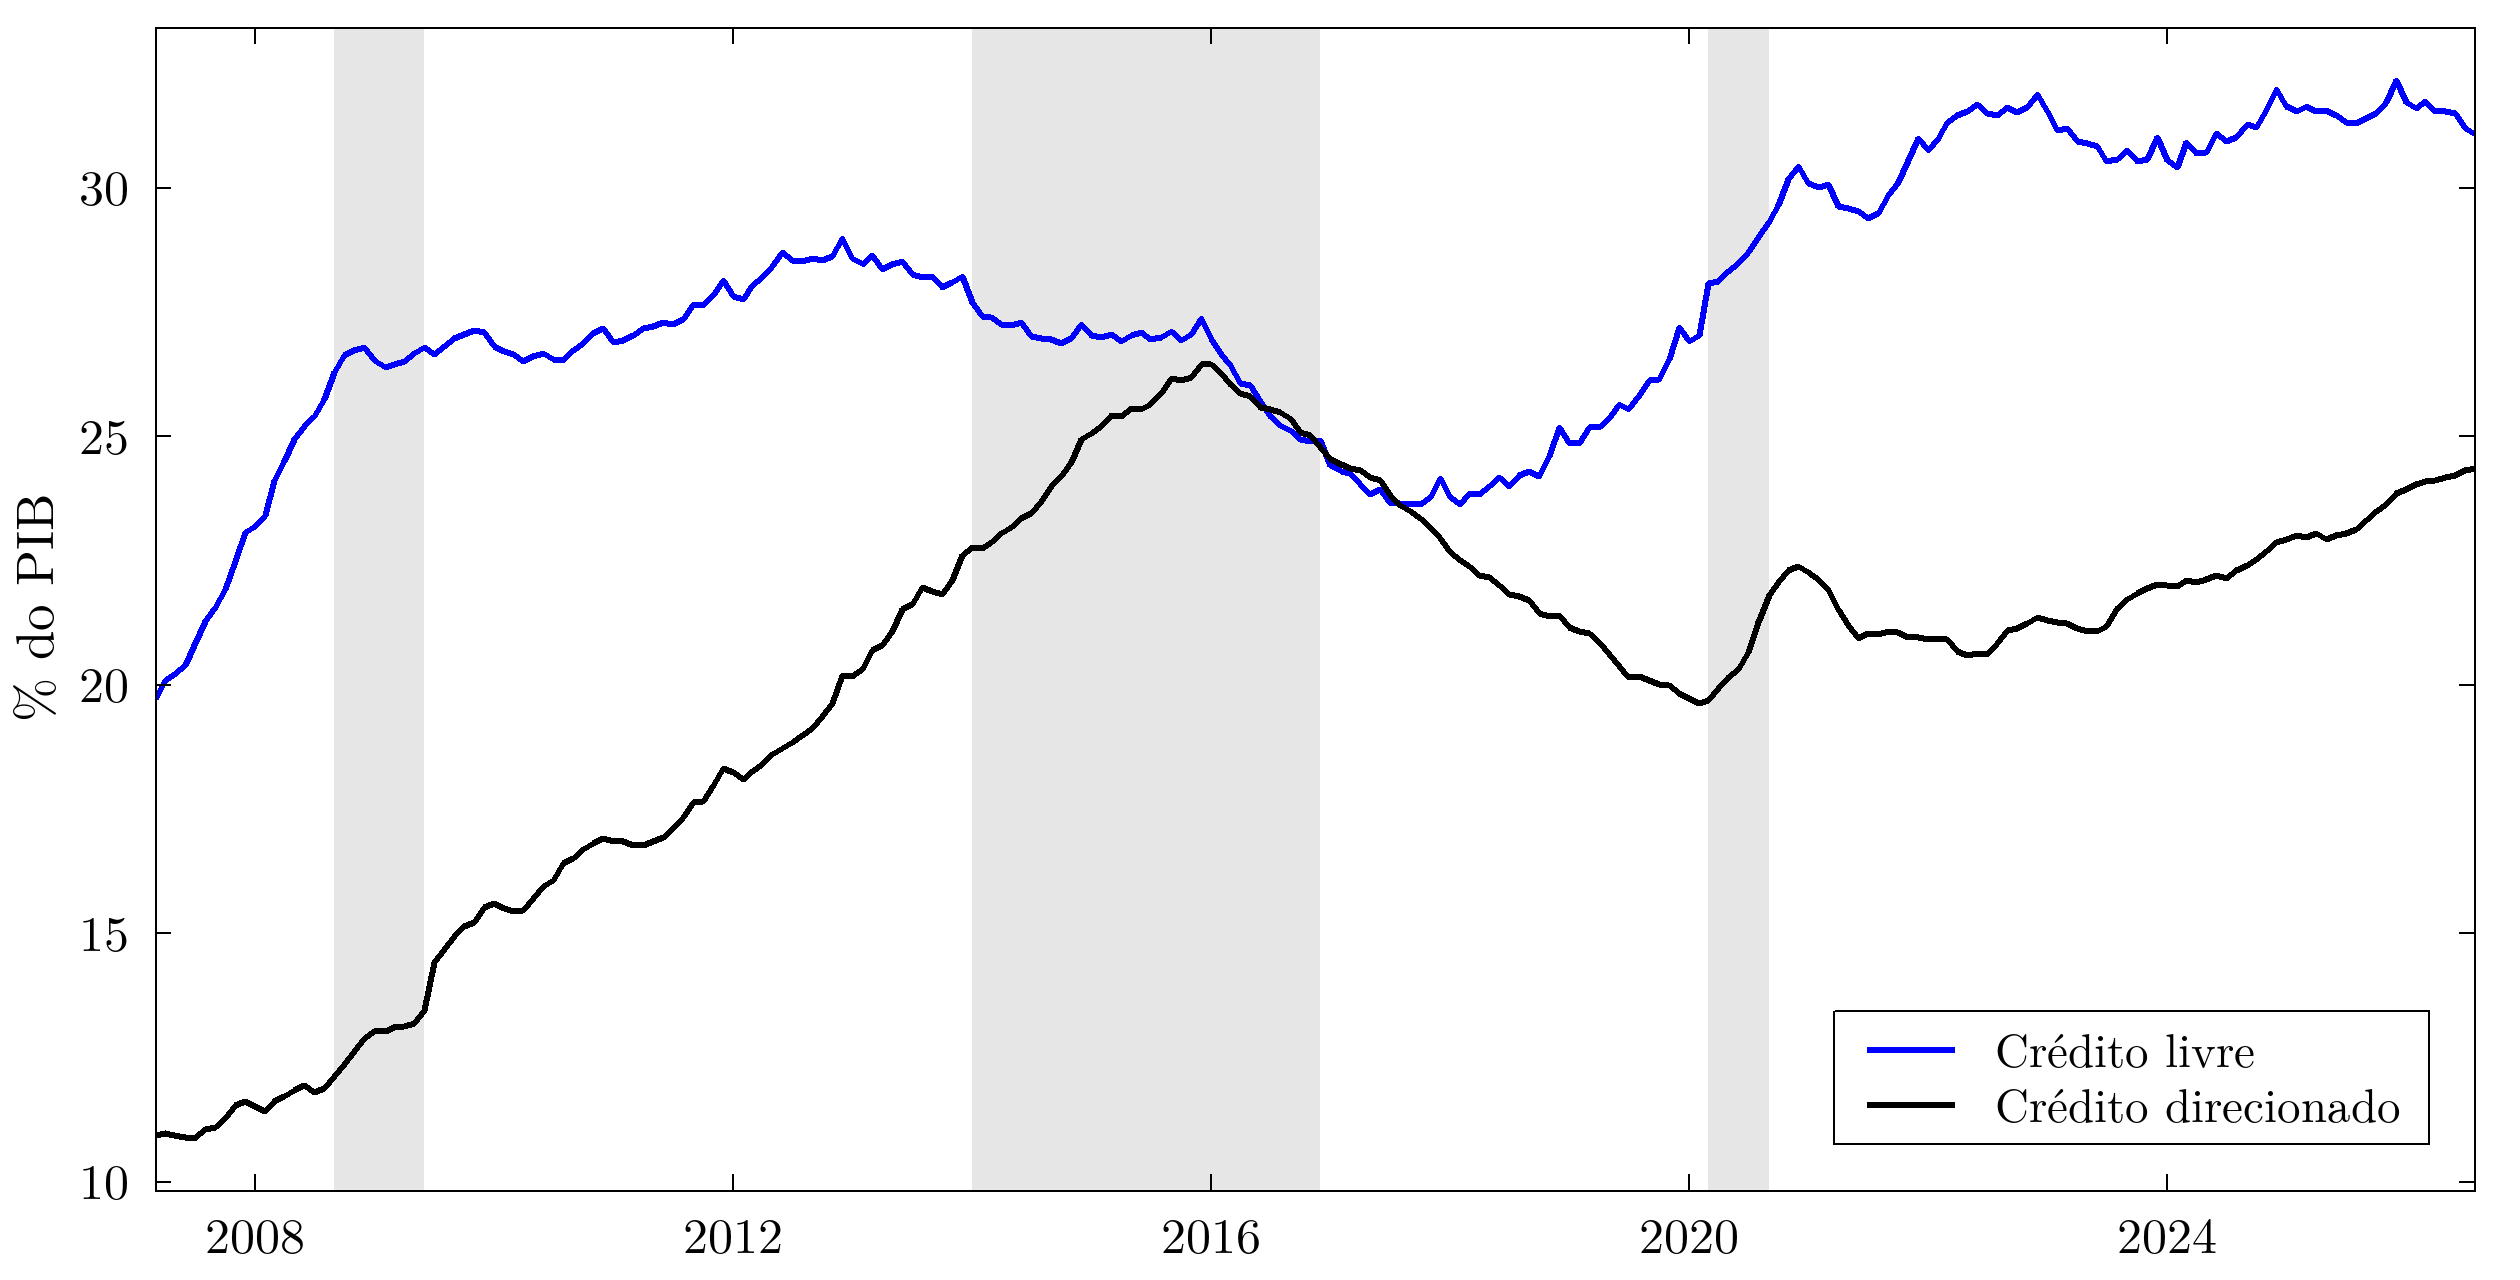
\includegraphics[width=\linewidth]{latex_fig02_livre_direcionado.png}
      \fonte{Crédito livre e direcionado (\% do PIB). Áreas sombreadas: recessões. Fonte: BCB (SGS).}
    \end{column}
    \begin{column}{0.42\textwidth}
      \small
      \begin{itemize}
        \item \textbf{Livre:} taxas pactuadas com o banco, que seguem a Selic e o risco
        \item \textbf{Direcionado:} habitação (poupança e FGTS), rural e BNDES, com taxas reguladas
        \item Após 2008, o direcionado cresce como \alert{política anticíclica}
        \item Crédito subsidiado tende a \alert{substituir} o livre (Bonomo, Brito e Martins, 2015)
      \end{itemize}
      \vspace{2pt}
      \reserva{r-concessoes}{Concessões por modalidade}
    \end{column}
  \end{columns}
\end{frame}

\begin{frame}[label=taxas]{O preço do crédito por segmento}
  \centering\small
  \begin{tabular}{@{}llrr@{}}
    \toprule
    Modalidade & Segmento & Dez./2016 & Jan./2023 \\
    \midrule
    Rotativo do cartão     & Livre PF        & 497,7 & 415,7 \\
    Cheque especial        & Livre PF        & 282,6 & 131,1 \\
    Pessoal não consignado & Livre PF        & 139,8 &  84,2 \\
    Consignado total       & Livre PF        &  29,4 &  26,7 \\
    Capital de giro        & Livre PJ        &  23,7 &  24,6 \\
    Habitacional (SFH)     & Direcionado PF  &  10,2 &  10,6 \\
    Crédito rural          & Direcionado PJ  &  11,5 &  13,7 \\
    \bottomrule
  \end{tabular}
  \fonte{Taxas médias de juros (\% a.a.). Selic a 13,75\% nas duas datas. Fonte: BCB (SGS).}
  \vspace{6pt}
  \raggedright
  Com a mesma Selic, as taxas livres vão de \alert{24\% a 498\%} ao ano, e as direcionadas ficam entre \alert{10\% e 14\%}\hfill\reserva{r-taxas}{Taxas ao longo do tempo}
\end{frame}

%==============================================================================
\section{Dados e metodologia}
%==============================================================================

\begin{frame}[label=dados]{Dados}
  \centering\small
  \begin{tabular}{@{}lll@{}}
    \toprule
    Variável & Definição & Unidade \\
    \midrule
    IBC-Br                      & Atividade econômica, com ajuste sazonal          & $100 \times \log$ \\
    IPCA                        & Índice de preços ao consumidor                   & $100 \times \log$ \\
    Saldo real do crédito livre & Saldo deflacionado pelo IPCA                     & $100 \times \log$ \\
    Meta Selic                  & Meta vigente no último dia do mês                & p.p. \\
    Spread do crédito livre     & Taxa das novas operações $-$ custo de captação   & p.p. \\
    Câmbio real efetivo         & Alta indica depreciação do real                  & $100 \times \log$ \\
    \bottomrule
  \end{tabular}\\[8pt]
  \raggedright
  \begin{itemize}
    \item Mensal, de mar./2011 a ago./2025 (\alert{174 observações}), do SGS do Banco Central
    \item Dummies sazonais e de eventos: recessão, greve de 2018, eleição, pandemia e crise fiscal de 2021
  \end{itemize}
  \vspace{2pt}
  \reserva{r-spread}{Definição do spread}\;
  \reserva{r-series}{Séries}\;
  \reserva{r-dummies}{Dummies}
\end{frame}

\begin{frame}[label=modelo]{Modelo e identificação}
  \vspace{-4pt}
  \[
    y_t = c + A_1 y_{t-1} + \dots + A_4 y_{t-4} + \Gamma D_t + u_t, \qquad u_t = B\,\varepsilon_t
  \]
  \vspace{-10pt}
  \begin{itemize}
    \item \alert{VAR em nível}, com 4 defasagens: não exige impor relações de cointegração (Sims, Stock e Watson, 1990)
    \item \alert{Ordenação recursiva} (Christiano, Eichenbaum e Evans, 1999): $B$ triangular inferior, por Cholesky
  \end{itemize}
  \vspace{2pt}
  \centering
  \usebeamercolor{structure}
  \begin{tikzpicture}[
      var/.style={draw=structure.fg, fill=structure.fg!8, rounded corners=2pt, minimum height=6mm, inner xsep=5pt, font=\small},
      pol/.style={var, fill=structure.fg, text=white, font=\small\bfseries},
      seta/.style={-{Stealth[length=2mm]}, structure.fg, thick}]
    \node[var] (ibc) {IBC-Br};
    \node[var, right=3mm of ibc] (ipca) {IPCA};
    \node[var, right=3mm of ipca] (saldo) {Saldo real};
    \node[pol, right=6mm of saldo] (meta) {Meta Selic};
    \node[var, right=6mm of meta] (spread) {Spread};
    \node[var, right=3mm of spread] (cambio) {Câmbio};
    \draw[seta] (saldo) -- (meta);
    \draw[seta] (meta) -- (spread);
    \node[below=1mm of ipca, font=\scriptsize, text=black!65] {não reagem à Selic no mês};
    \node[below=1mm of spread.south east, anchor=north, font=\scriptsize, text=black!65] {reagem no mesmo mês};
  \end{tikzpicture}\\[4pt]
  \raggedright\small
  Choque de 1 desvio-padrão na meta $=$ \alert{0,29 p.p.} \quad IC de 95\% por bootstrap, com 5.000 réplicas\\[4pt]
  \reserva{r-testes}{Raiz unitária e cointegração}\;
  \reserva{r-defasagens}{Defasagens}\;
  \reserva{r-ordem}{Outras ordenações}\;
  \reserva{r-choque}{Choque de 1 p.p.}
\end{frame}

\begin{frame}{Verificação por projeções locais}
  \[
    y_{i,t+h} - y_{i,t-1} = \alpha_h + \beta_h\, \varepsilon_t + \gamma_h' X_t + e_{t+h}, \qquad h = 0, \dots, 24
  \]
  \begin{itemize}
    \item Uma regressão por horizonte (Jordà, 2005): $\beta_h$ é a resposta $h$ meses após o choque
    \item Mesmo choque e mesma hipótese de identificação do VAR; $X_t$ reúne controles, 4 defasagens e as dummies
    \item Não depende de a dinâmica do VAR estar bem especificada
    \item Erros-padrão de Newey e West (1987), robustos à \alert{autocorrelação} que o teste do sistema ainda acusa no VAR
  \end{itemize}
\end{frame}

%==============================================================================
\section{Resultados}
%==============================================================================

\begin{frame}[label=resultado1]{Resultado 1: o preço do crédito reage}
  \begin{columns}[T]
    \begin{column}{0.60\textwidth}
      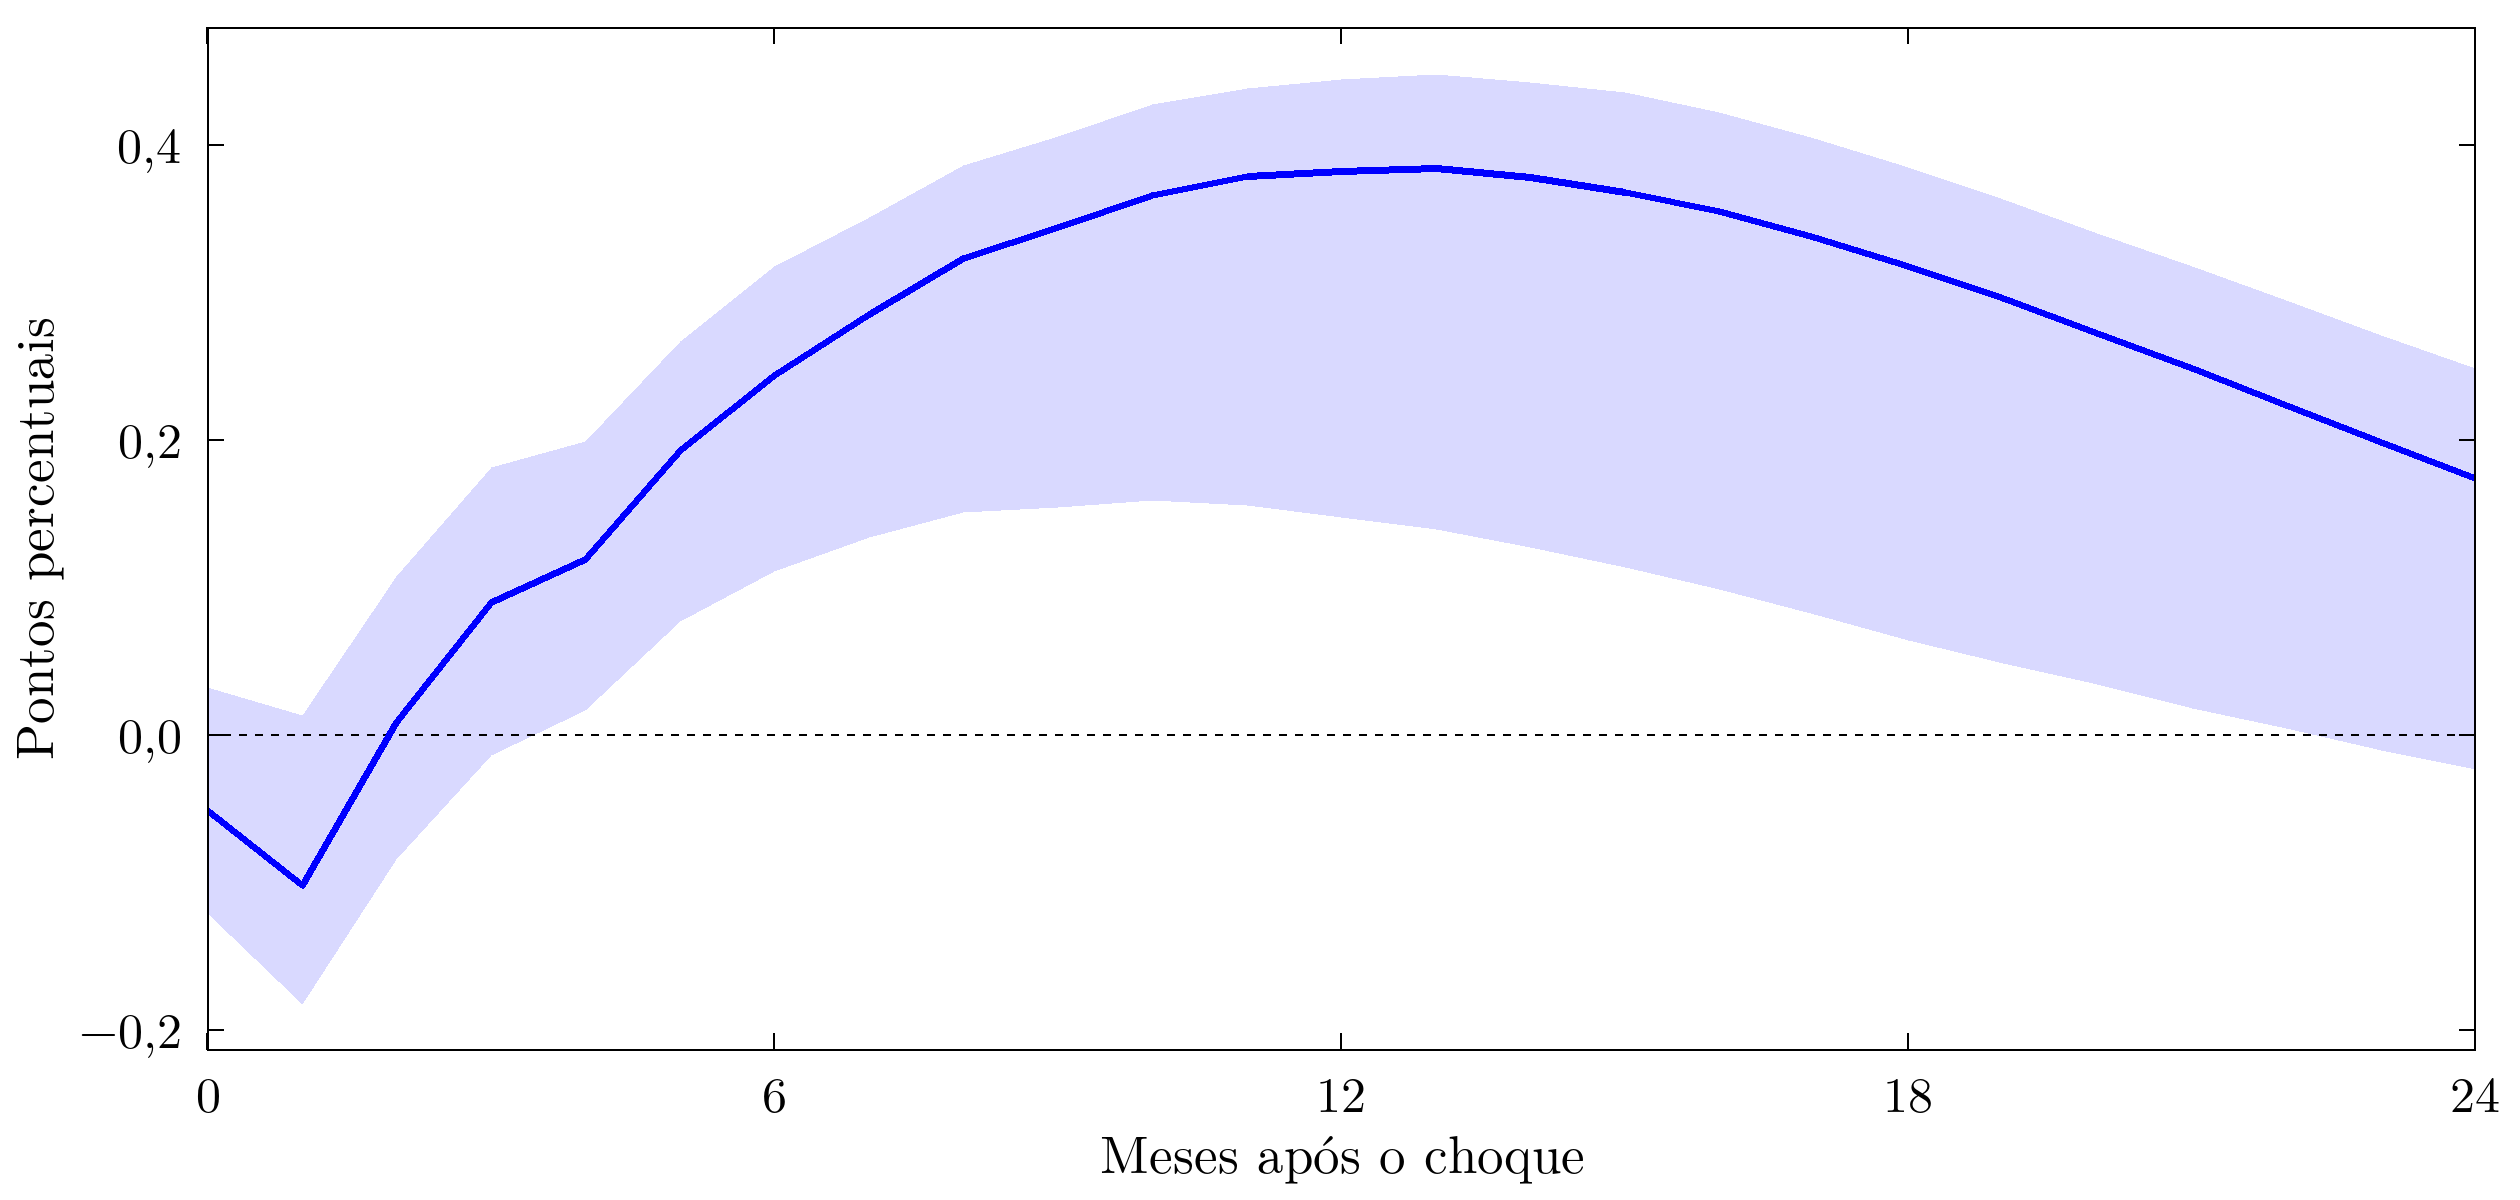
\includegraphics[width=\linewidth]{latex_fig07_irf_spread.png}
      \fonte{Resposta do spread (p.p.) a um choque de 1 d.p. na meta Selic. IC de 95\%, bootstrap com 5.000 réplicas.}
    \end{column}
    \begin{column}{0.38\textwidth}
      \small
      \begin{itemize}
        \item Sobe a partir do \alert{4º mês} e segue significativo até o 22º
        \item Pico de \alert{0,38 p.p.} perto de um ano, quando a meta está 0,32 p.p. acima do início
        \item Como o spread é medido sobre o custo de captação, a taxa ao tomador sobe \alert{mais} que o custo do banco
        \item É o \alert{prêmio de financiamento externo} da teoria
      \end{itemize}
      \reserva{r-longo}{Horizonte de 120 meses}
    \end{column}
  \end{columns}
\end{frame}

\begin{frame}{Resultado 2: a quantidade reage menos}
  \begin{columns}[c]
    \begin{column}{0.48\textwidth}
      \centering
      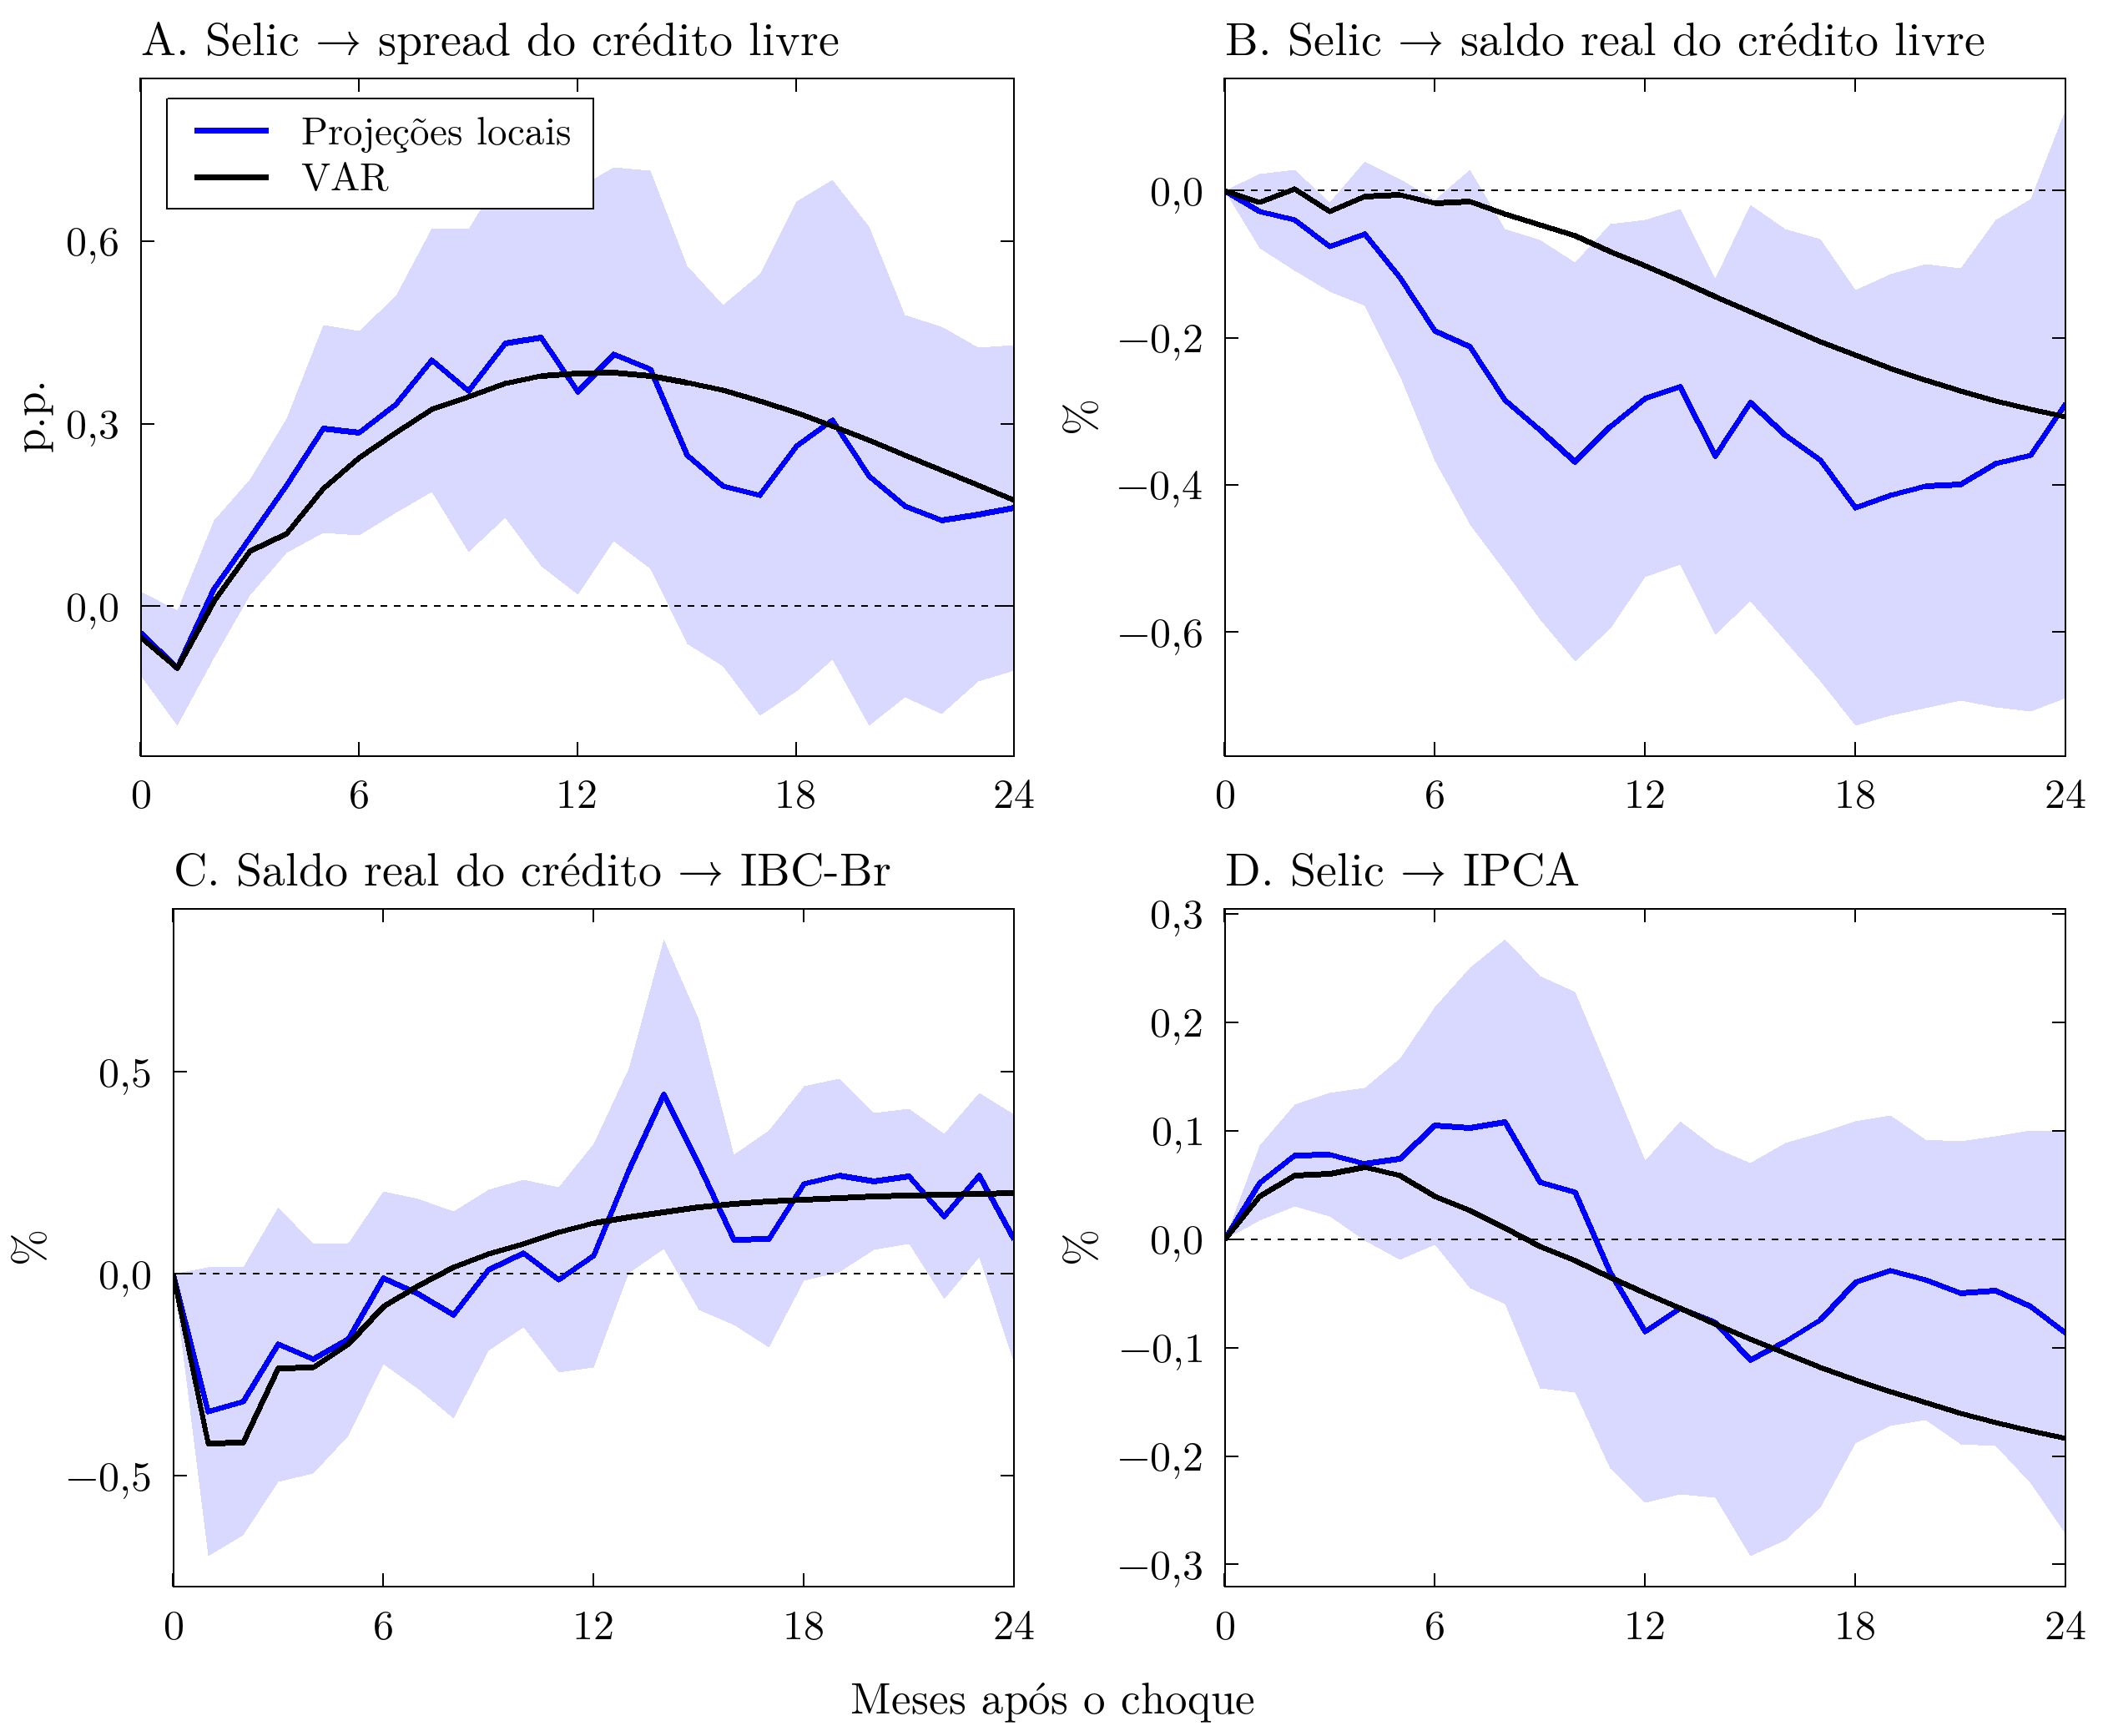
\includegraphics[width=\linewidth]{latex_fig09_lp_vs_var.png}
    \end{column}
    \begin{column}{0.48\textwidth}
      \small
      \begin{itemize}
        \item No VAR, o saldo cai \alert{0,10\%} em um ano e \alert{0,31\%} em dois, sem significância
        \item Nas projeções locais, a queda chega a cerca de \alert{0,4\%} e é significativa do 8º ao 23º mês (painel B)
        \item As projeções locais confirmam a alta do spread (painel A)
        \item A Selic explica \alert{38\%} da variância do spread em dois anos, mas menos de \alert{3\%} da do saldo
      \end{itemize}
      \fonte{Azul: projeções locais, com IC de 95\% (Newey-West). Preto: VAR.}
    \end{column}
  \end{columns}
\end{frame}

\begin{frame}{Resultado 3: o crédito importa para a atividade}
  \begin{columns}[T]
    \begin{column}{0.60\textwidth}
      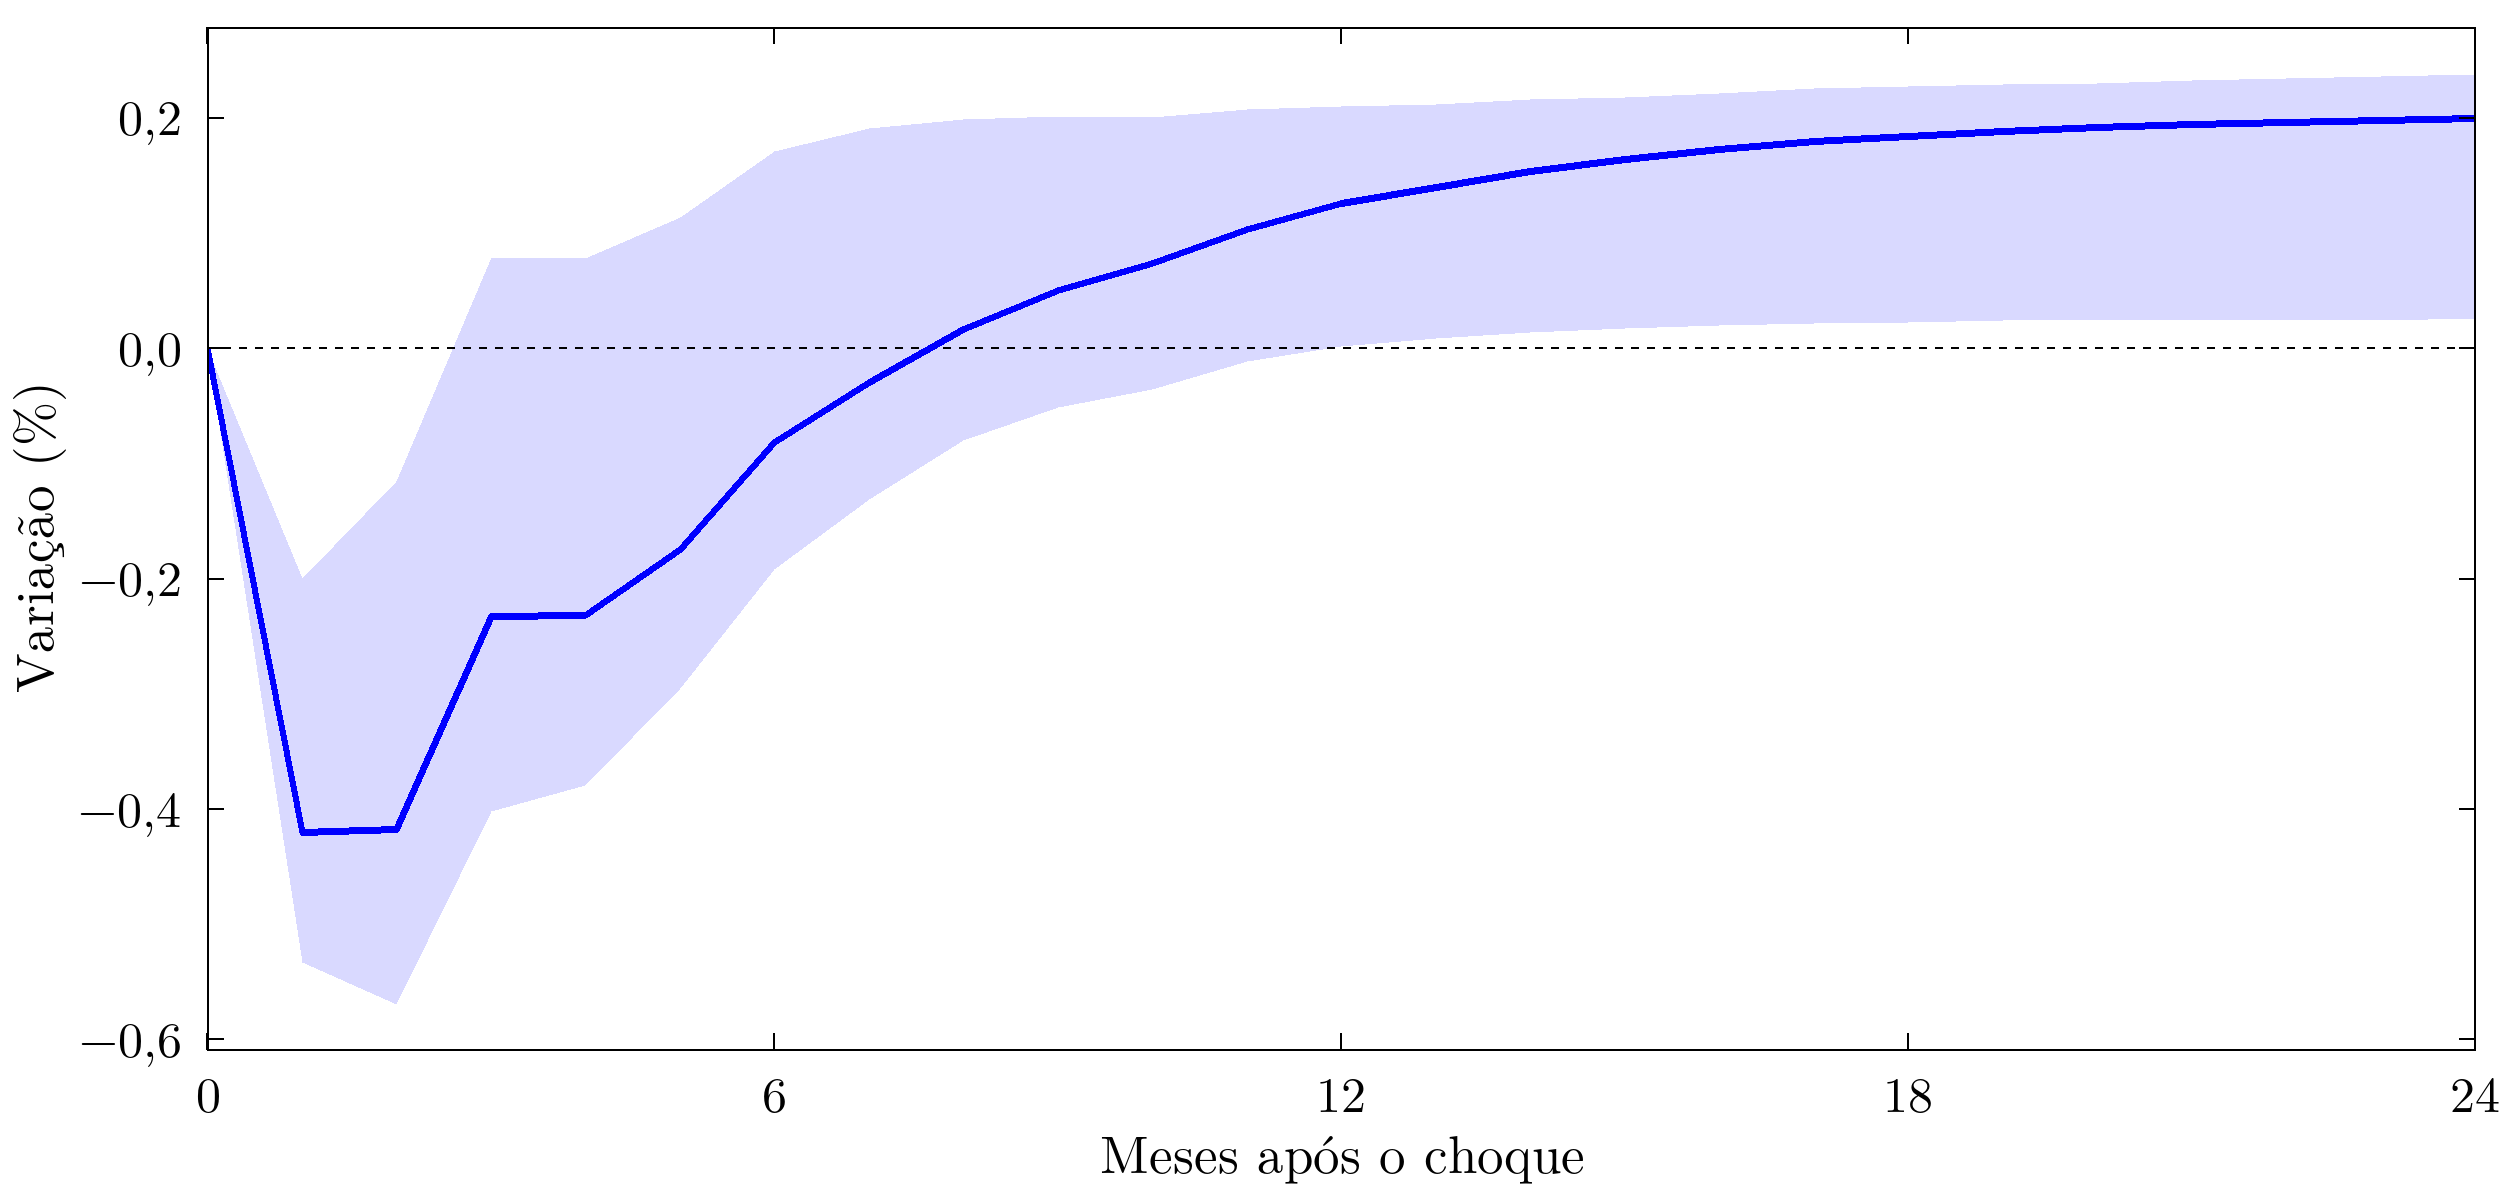
\includegraphics[width=\linewidth]{latex_fig10_irf_saldo_ibc.png}
      \fonte{Resposta do IBC-Br (\%) a um choque de 1 d.p. no saldo real do crédito livre. IC de 95\%, bootstrap com 5.000 réplicas.}
    \end{column}
    \begin{column}{0.38\textwidth}
      \small
      \begin{itemize}
        \item Mais crédito eleva o IBC-Br entre o \alert{12º e o 24º mês}, cerca de 0,2\% no fim
        \item A queda nos dois primeiros meses é compatível com a demanda por capital de giro quando o faturamento cai (Den Haan, Sumner e Yamashiro, 2007)
        \item Mede a relação dinâmica entre crédito e atividade, e \alert{não} um efeito puro da oferta de crédito
      \end{itemize}
    \end{column}
  \end{columns}
\end{frame}

\begin{frame}[label=fevd]{Decomposição da variância}
  \begin{columns}[c]
    \begin{column}{0.56\textwidth}
      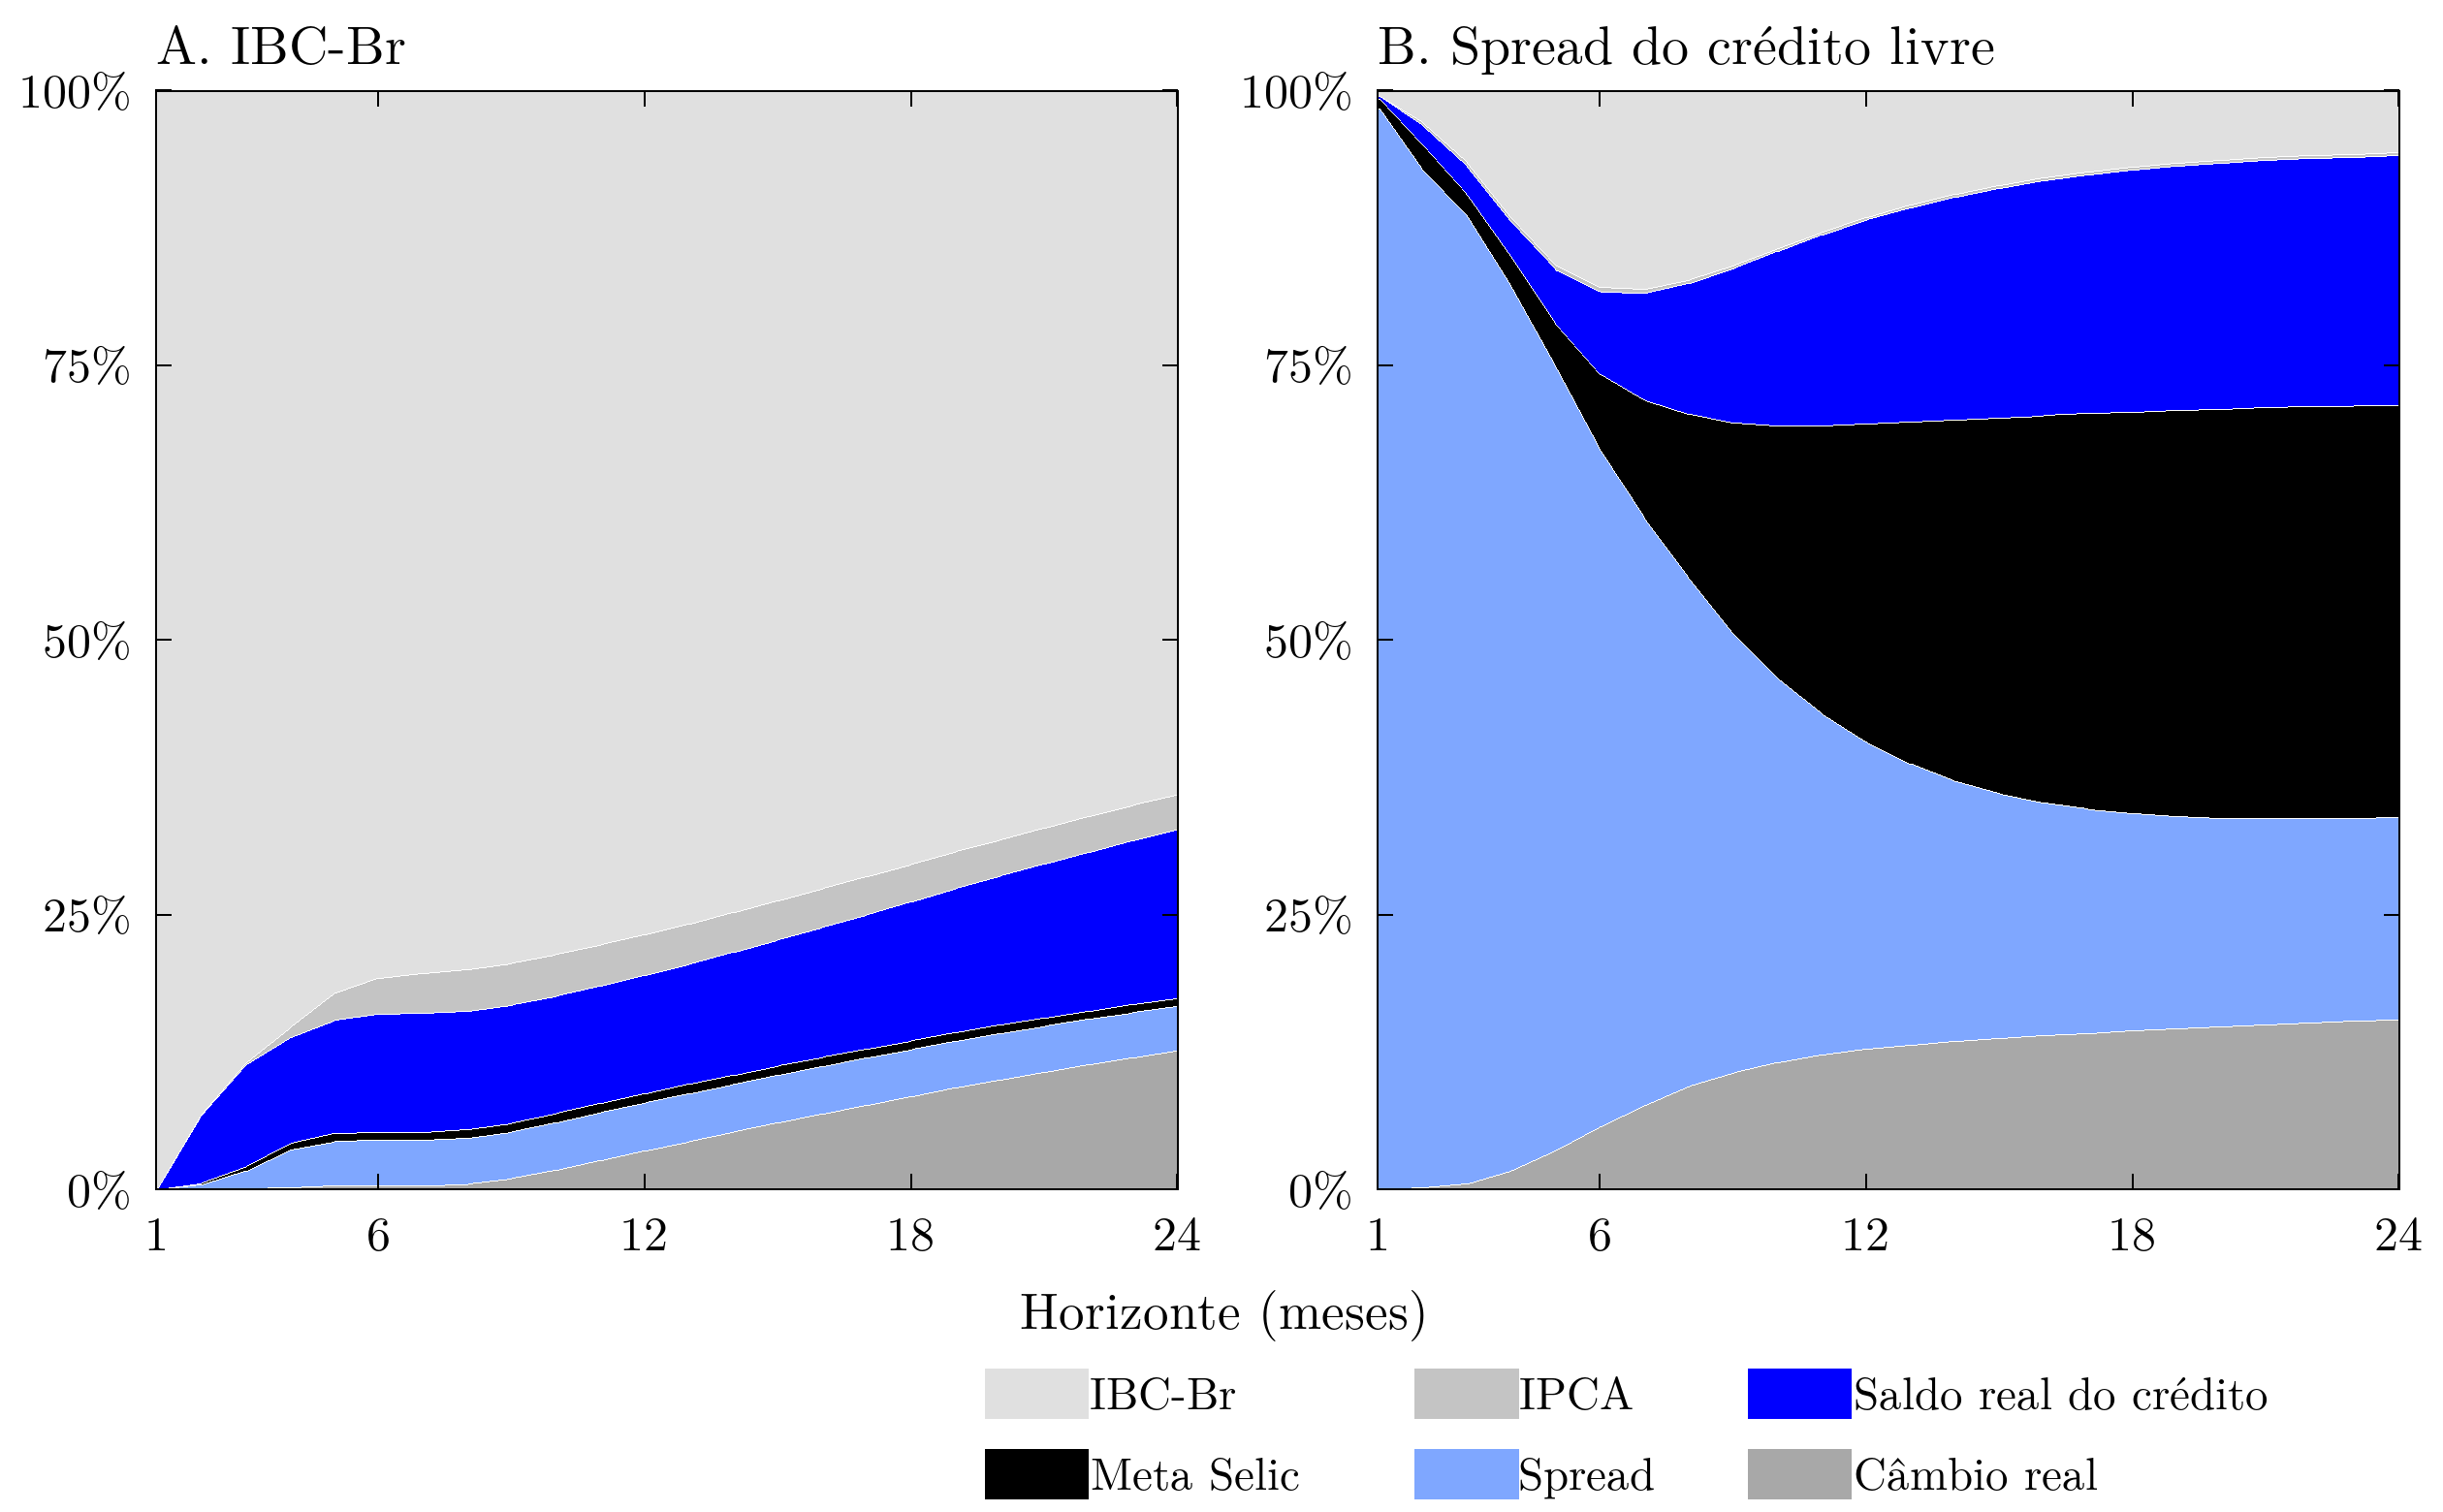
\includegraphics[width=\linewidth]{latex_fig_fevd.png}
      \fonte{Parcela da variância do erro de previsão explicada por choques em cada variável, por horizonte.}
    \end{column}
    \begin{column}{0.42\textwidth}
      \small
      \begin{itemize}
        \item O crédito livre explica \alert{15\%} da variância do IBC-Br em dois anos
        \item Mais que o câmbio (13\%) e muito mais que a Selic (\alert{menos de 1\%})
        \item O efeito direto da Selic sobre o IBC-Br \alert{não é significativo} em nenhum horizonte
        \item Não é ausência de transmissão: o efeito líquido não se distingue de zero
      \end{itemize}
      \vspace{2pt}
      \reserva{r-fevd}{Tabela}\;
      \reserva{r-compl}{Outras respostas}
    \end{column}
  \end{columns}
\end{frame}

\begin{frame}[label=segmentos]{O teste da segmentação: livre e direcionado}
  \centering
  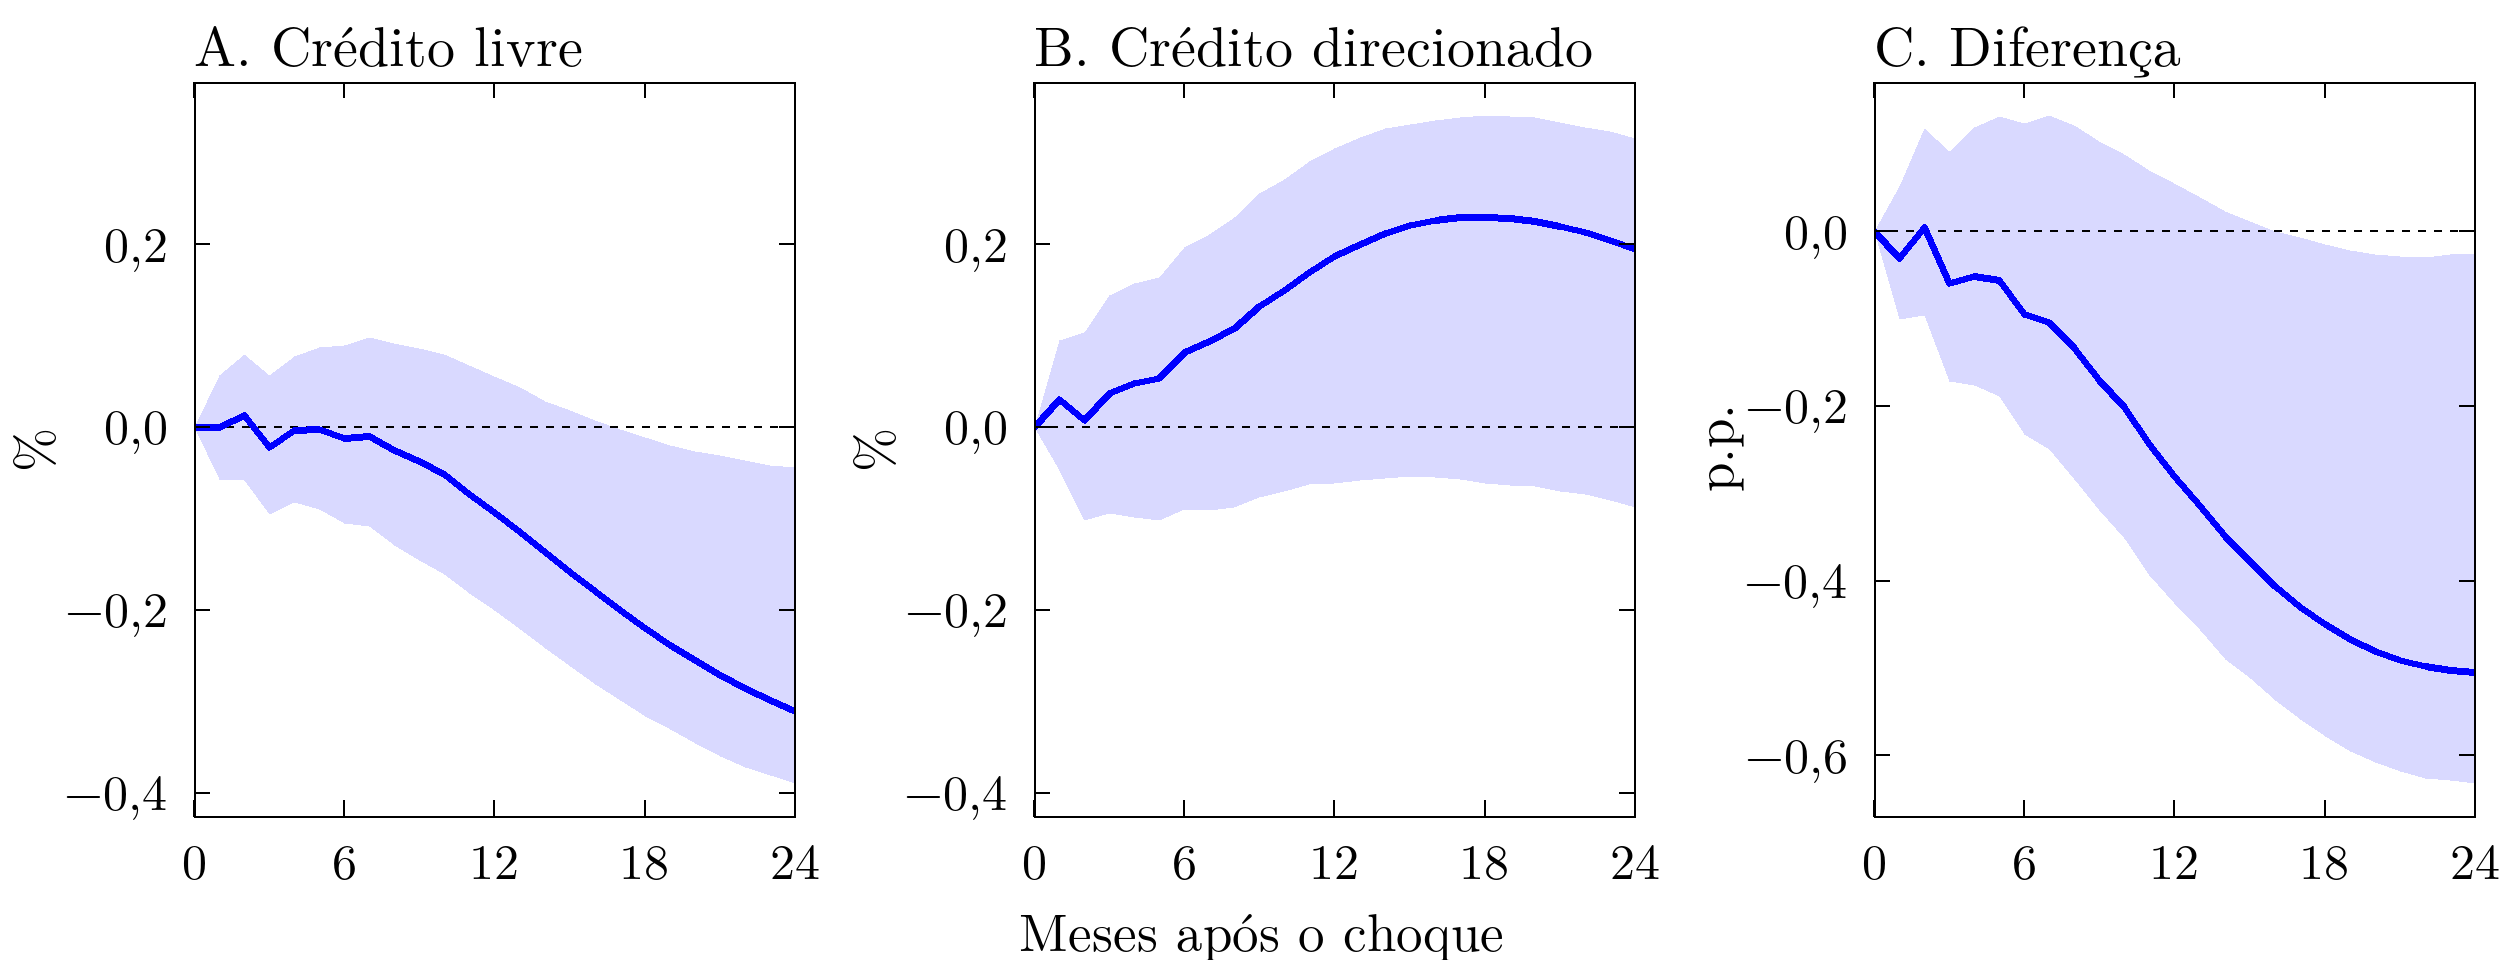
\includegraphics[width=0.76\textwidth]{latex_fig12_livre_direcionado.png}
  \fonte{Saldos reais (\%) após choque de 1 d.p. na meta Selic, no mesmo VAR. IC de 95\%, bootstrap com 5.000 réplicas.}
  \vspace{2pt}
  \raggedright\small
  \begin{itemize}
    \item Os dois saldos no \alert{mesmo modelo}, com a mesma amostra, defasagens e ordenação
    \item O livre cai do 17º ao 24º mês ($-$0,31\%); o \alert{direcionado não responde}; a \alert{diferença} é significativa a partir do 17º mês
  \end{itemize}
  \vspace{-2pt}\hfill\reserva{r-direcionado}{Robustez}
\end{frame}

\begin{frame}{Crédito total e substituição}
  \begin{columns}[T]
    \begin{column}{0.58\textwidth}
      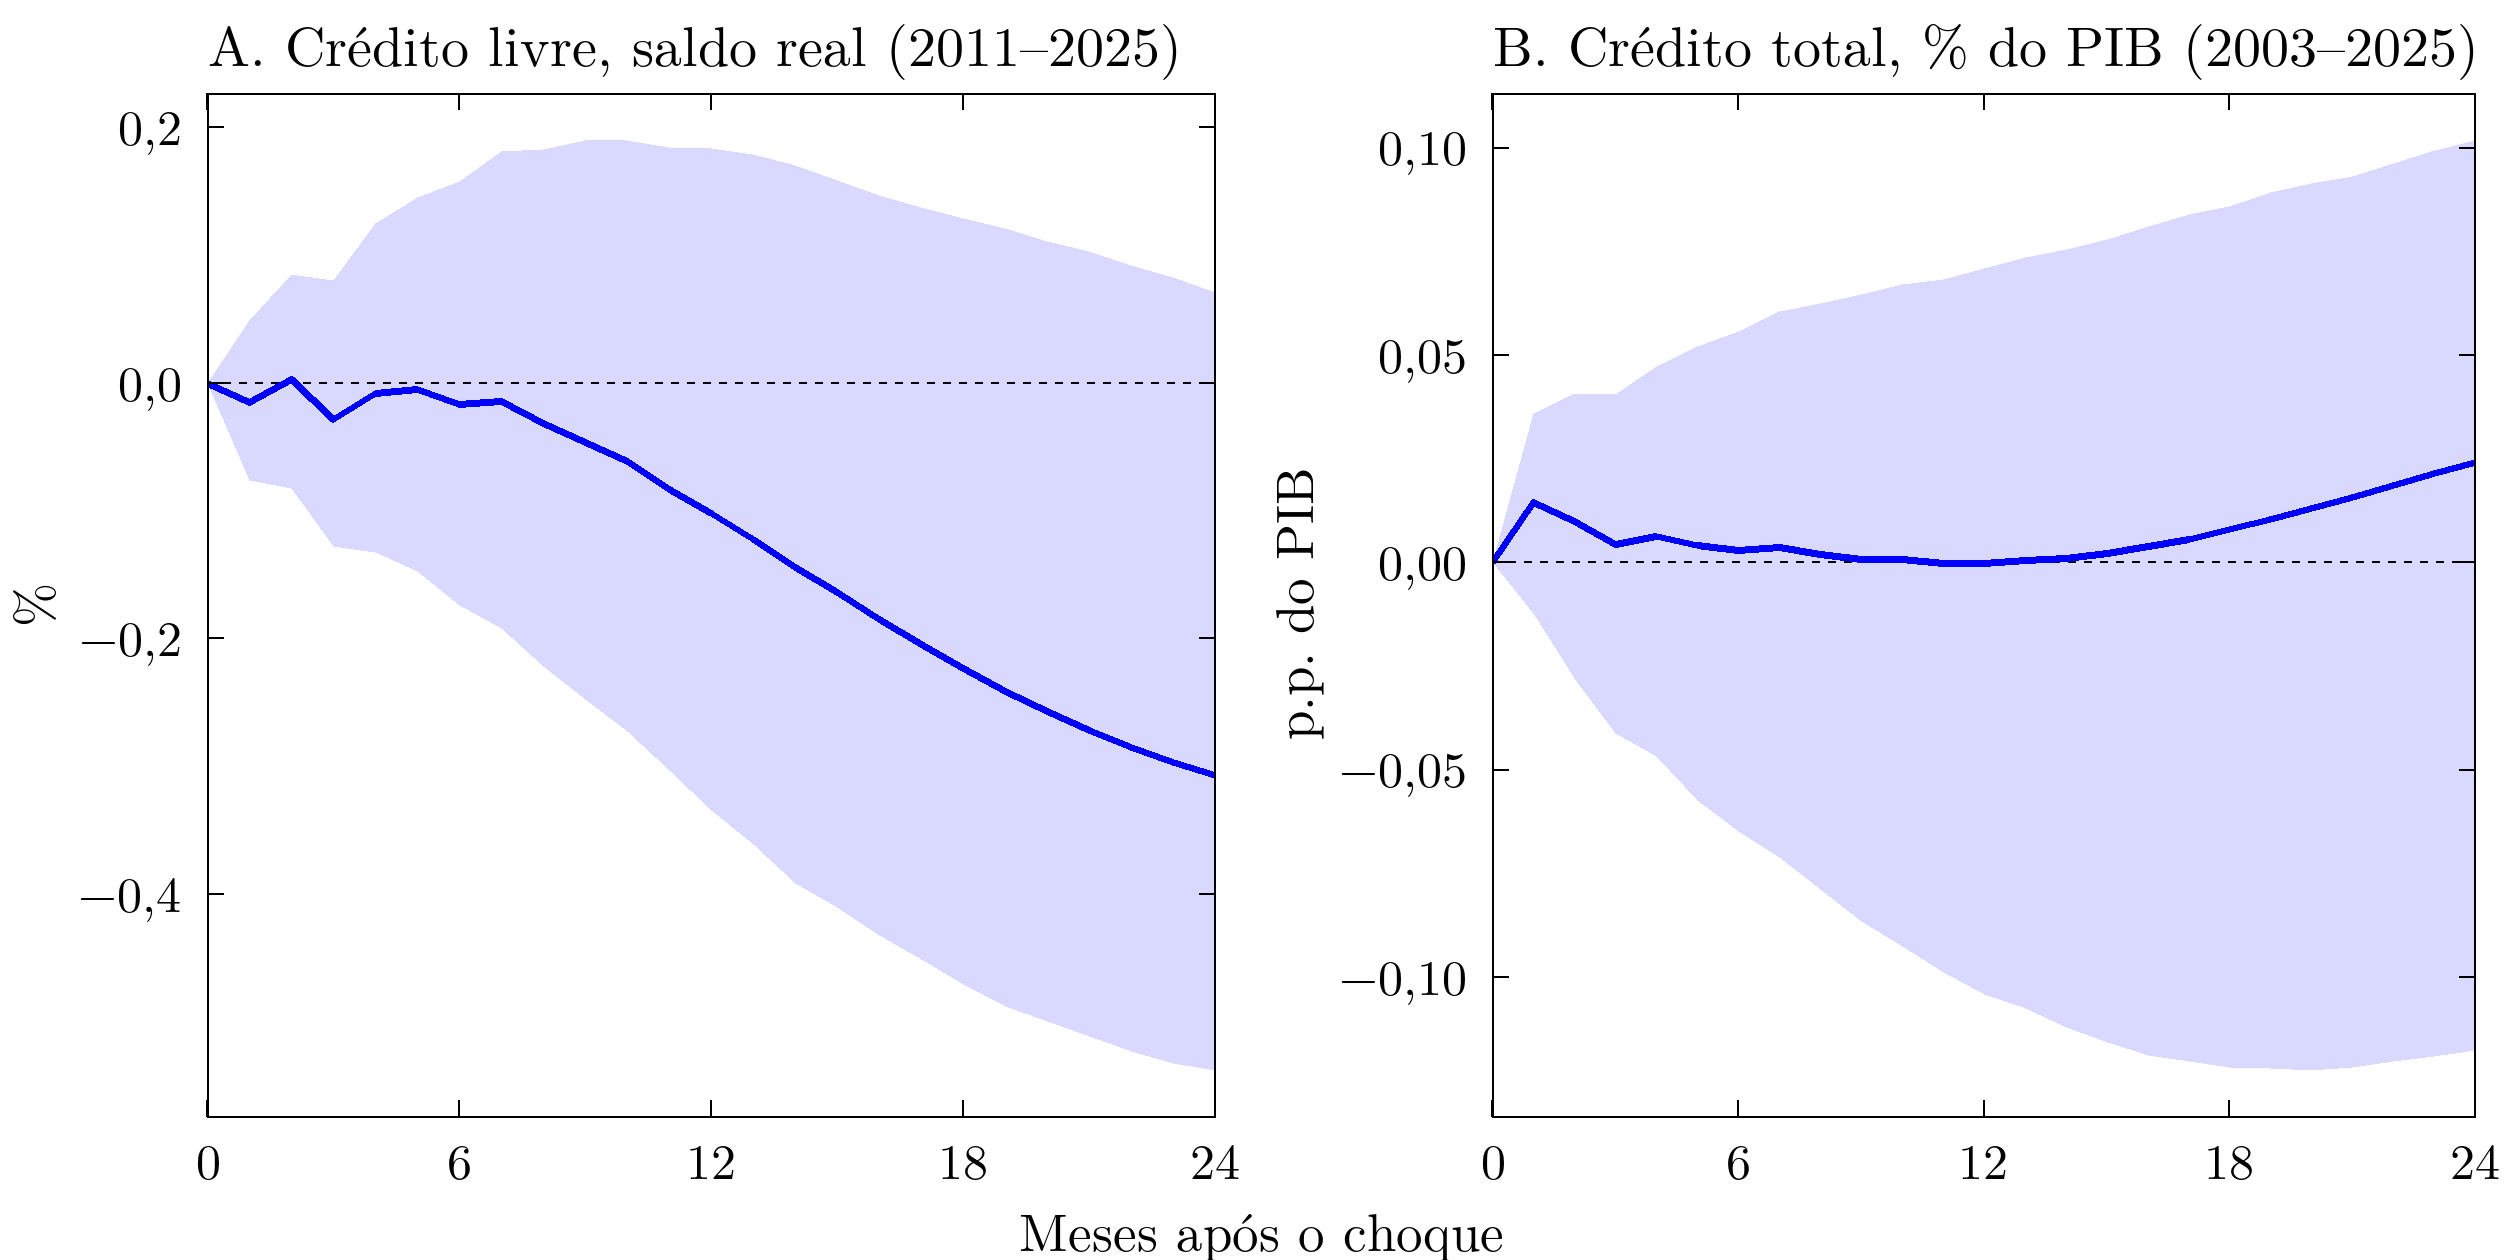
\includegraphics[width=\linewidth]{latex_fig13_livre_total.png}
      \fonte{A: saldo real do crédito livre, modelo principal (2011--2025). B: crédito total em \% do PIB (2003--2025). Choque de 1 d.p. na meta Selic de cada modelo.}
    \end{column}
    \begin{column}{0.40\textwidth}
      \small
      \begin{itemize}
        \item Com o \alert{crédito total}, que inclui o direcionado, a resposta do volume à Selic \alert{desaparece}
        \item Choques no crédito direcionado \alert{elevam o IBC-Br}: parte do crédito que importa para o produto escapa da Selic
        \item Coerente com Leigh e Xu (2025), que chegam à mesma conclusão pelas taxas
      \end{itemize}
    \end{column}
  \end{columns}
\end{frame}

%==============================================================================
\section{Conclusão}
%==============================================================================

\begin{frame}{Implicações de política}
  \begin{itemize}
    \item Cada ponto de Selic alcança uma \alert{fração menor} da economia do que num mercado menos segmentado
    \item Para obter o mesmo efeito sobre a demanda, o Banco Central tende a precisar de ciclos de aperto \alert{mais longos ou mais intensos}
    \item O ajuste recai de forma desproporcional sobre os \alert{tomadores do crédito livre}, que pagam spreads maiores
    \item O crédito direcionado é uma fonte de demanda \alert{fora do alcance da Selic}
    \begin{itemize}
      \item Reduzir sua participação, como na transição da TJLP para a TLP, aumenta a potência da política monetária
      \item Expandi-lo durante um aperto a enfraquece
    \end{itemize}
  \end{itemize}
\end{frame}

\begin{frame}{Limitações e extensões}
  \begin{columns}[T]
    \begin{column}{0.49\textwidth}
      \begin{block}{Limitações}
        \small
        \begin{itemize}
          \item Amostra curta, imposta pela série de spread: 42 parâmetros por equação e 128 graus de liberdade
          \item Identificação recursiva, embora os resultados se mantenham sob outras ordenações
          \item O choque no saldo não separa oferta e demanda de crédito
        \end{itemize}
      \end{block}
    \end{column}
    \begin{column}{0.49\textwidth}
      \begin{block}{Extensões}
        \small
        \begin{itemize}
          \item Separar o crédito livre a famílias e a empresas
          \item Identificar a política monetária por surpresas de alta frequência (Elias e Guimarães, 2024), usadas como instrumento
        \end{itemize}
      \end{block}
    \end{column}
  \end{columns}
\end{frame}

\begin{frame}{Conclusão}
  \small
  \textbf{Objetivo:} verificar se a Selic afeta o custo e o volume do crédito livre e, por meio dele, a atividade\\[6pt]
  \centering
  \usebeamercolor{structure}
  \begin{tikzpicture}[
      elo/.style={draw=structure.fg, fill=structure.fg!8, rounded corners=3pt, align=center, text width=2.9cm, minimum height=0.95cm, font=\footnotesize,
                  execute at begin node={\hyphenpenalty=10000}},
      selic/.style={elo, fill=structure.fg, text=white, font=\footnotesize\bfseries, text width=1.6cm},
      fora/.style={elo, draw=black!40, fill=black!5, text=black!70},
      seta/.style={-{Stealth[length=2.2mm]}, structure.fg, thick}]
    \node[selic] (s) {Aperto monetário};
    \node[elo, right=5mm of s] (p) {Spread do crédito livre\\\alert{sobe}};
    \node[elo, right=5mm of p] (q) {Volume do crédito livre\\\alert{cai, com atraso}};
    \node[elo, right=5mm of q] (a) {Atividade\\crédito explica \alert{15\%}};
    \node[fora, below=3mm of q] (d) {Crédito direcionado\\não responde};
    \draw[seta] (s) -- (p);
    \draw[seta] (p) -- (q);
    \draw[seta] (q) -- (a);
    \draw[seta, black!40, dashed] (s.south) |- (d.west) node[pos=0.75, above, font=\scriptsize, text=black!60] {sem efeito};
  \end{tikzpicture}\\[6pt]
  \begin{block}{Resposta à pergunta}
    O canal de crédito opera no Brasil, mas só sobre a parcela livre do mercado: a segmentação entre crédito livre e direcionado o \alert{obstrui parcialmente}.
  \end{block}
\end{frame}

\begin{frame}[plain]
  \centering
  \vfill
  {\usebeamercolor[fg]{structure}\Huge Obrigado!}\\[14pt]
  {\large João Victor Alonso Kutianski Santana}\\[4pt]
  {\small Instituto de Economia -- UFRJ}\\[16pt]
  \hyperlink{reservas}{\beamerskipbutton{Slides de reserva}}
  \vfill
\end{frame}

%==============================================================================
% RESERVA (fora da contagem de slides)
%==============================================================================
\appendix

\begin{frame}[label=reservas]{Slides de reserva}
  \begin{columns}[T]
    \begin{column}{0.49\textwidth}
      \textbf{Modelo}\\[4pt]
      \reserva{r-longo}{Respostas em 120 meses}\\[3pt]
      \reserva{r-ordem}{Outras ordenações}\\[3pt]
      \reserva{r-testes}{Raiz unitária e cointegração}\\[3pt]
      \reserva{r-defasagens}{Defasagens e autocorrelação}\\[3pt]
      \reserva{r-choque}{Choque de 1 p.p.}\\[3pt]
      \reserva{r-dummies}{Dummies}
    \end{column}
    \begin{column}{0.49\textwidth}
      \textbf{Dados e resultados}\\[4pt]
      \reserva{r-mecanismos}{Canais de transmissão}\\[3pt]
      \reserva{r-spread}{Definição do spread}\\[3pt]
      \reserva{r-series}{Séries do modelo}\\[3pt]
      \reserva{r-fevd}{Tabela da decomposição da variância}\\[3pt]
      \reserva{r-compl}{Respostas complementares}\\[3pt]
      \reserva{r-direcionado}{Robustez: livre e direcionado}\\[3pt]
      \reserva{r-taxas}{Taxas por segmento}\\[3pt]
      \reserva{r-concessoes}{Concessões do direcionado}
    \end{column}
  \end{columns}
\end{frame}

\begin{frame}[label=r-mecanismos]{Canais de transmissão da política monetária}
  \centering
  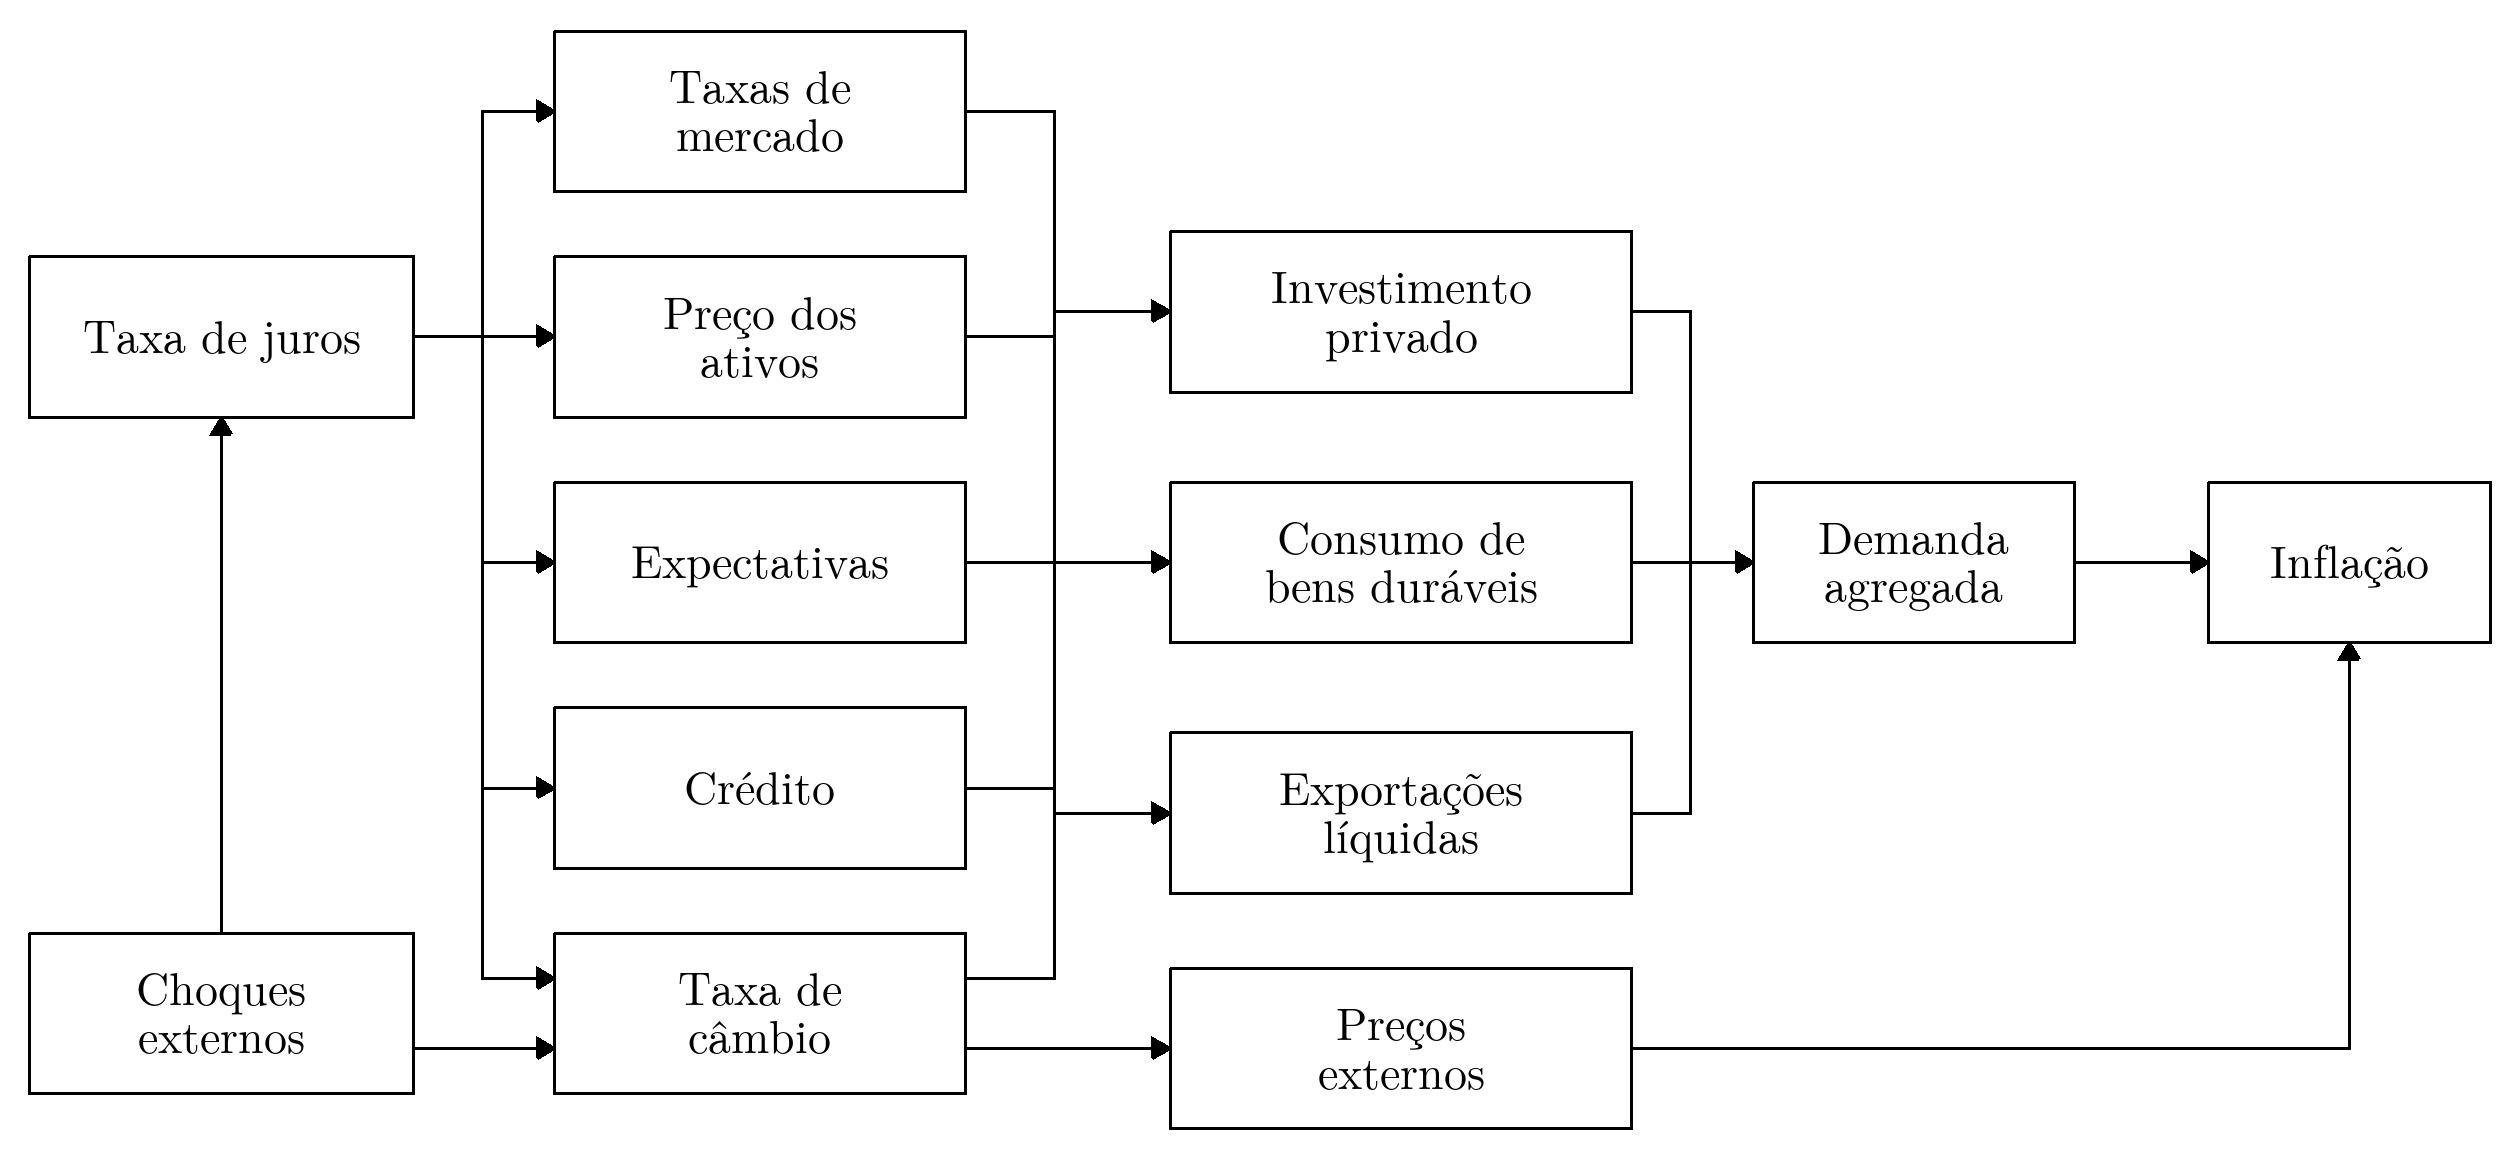
\includegraphics[width=0.74\textwidth]{latex_fig01_mecanismos.png}
  \fonte{Fonte: adaptado de Marcatti (2011).}
  \vspace{4pt}
  \raggedright
  \voltar{teoria}{Canal de crédito}\indicereserva
\end{frame}

\begin{frame}[label=r-longo]{Respostas em horizonte de 120 meses}
  \centering
  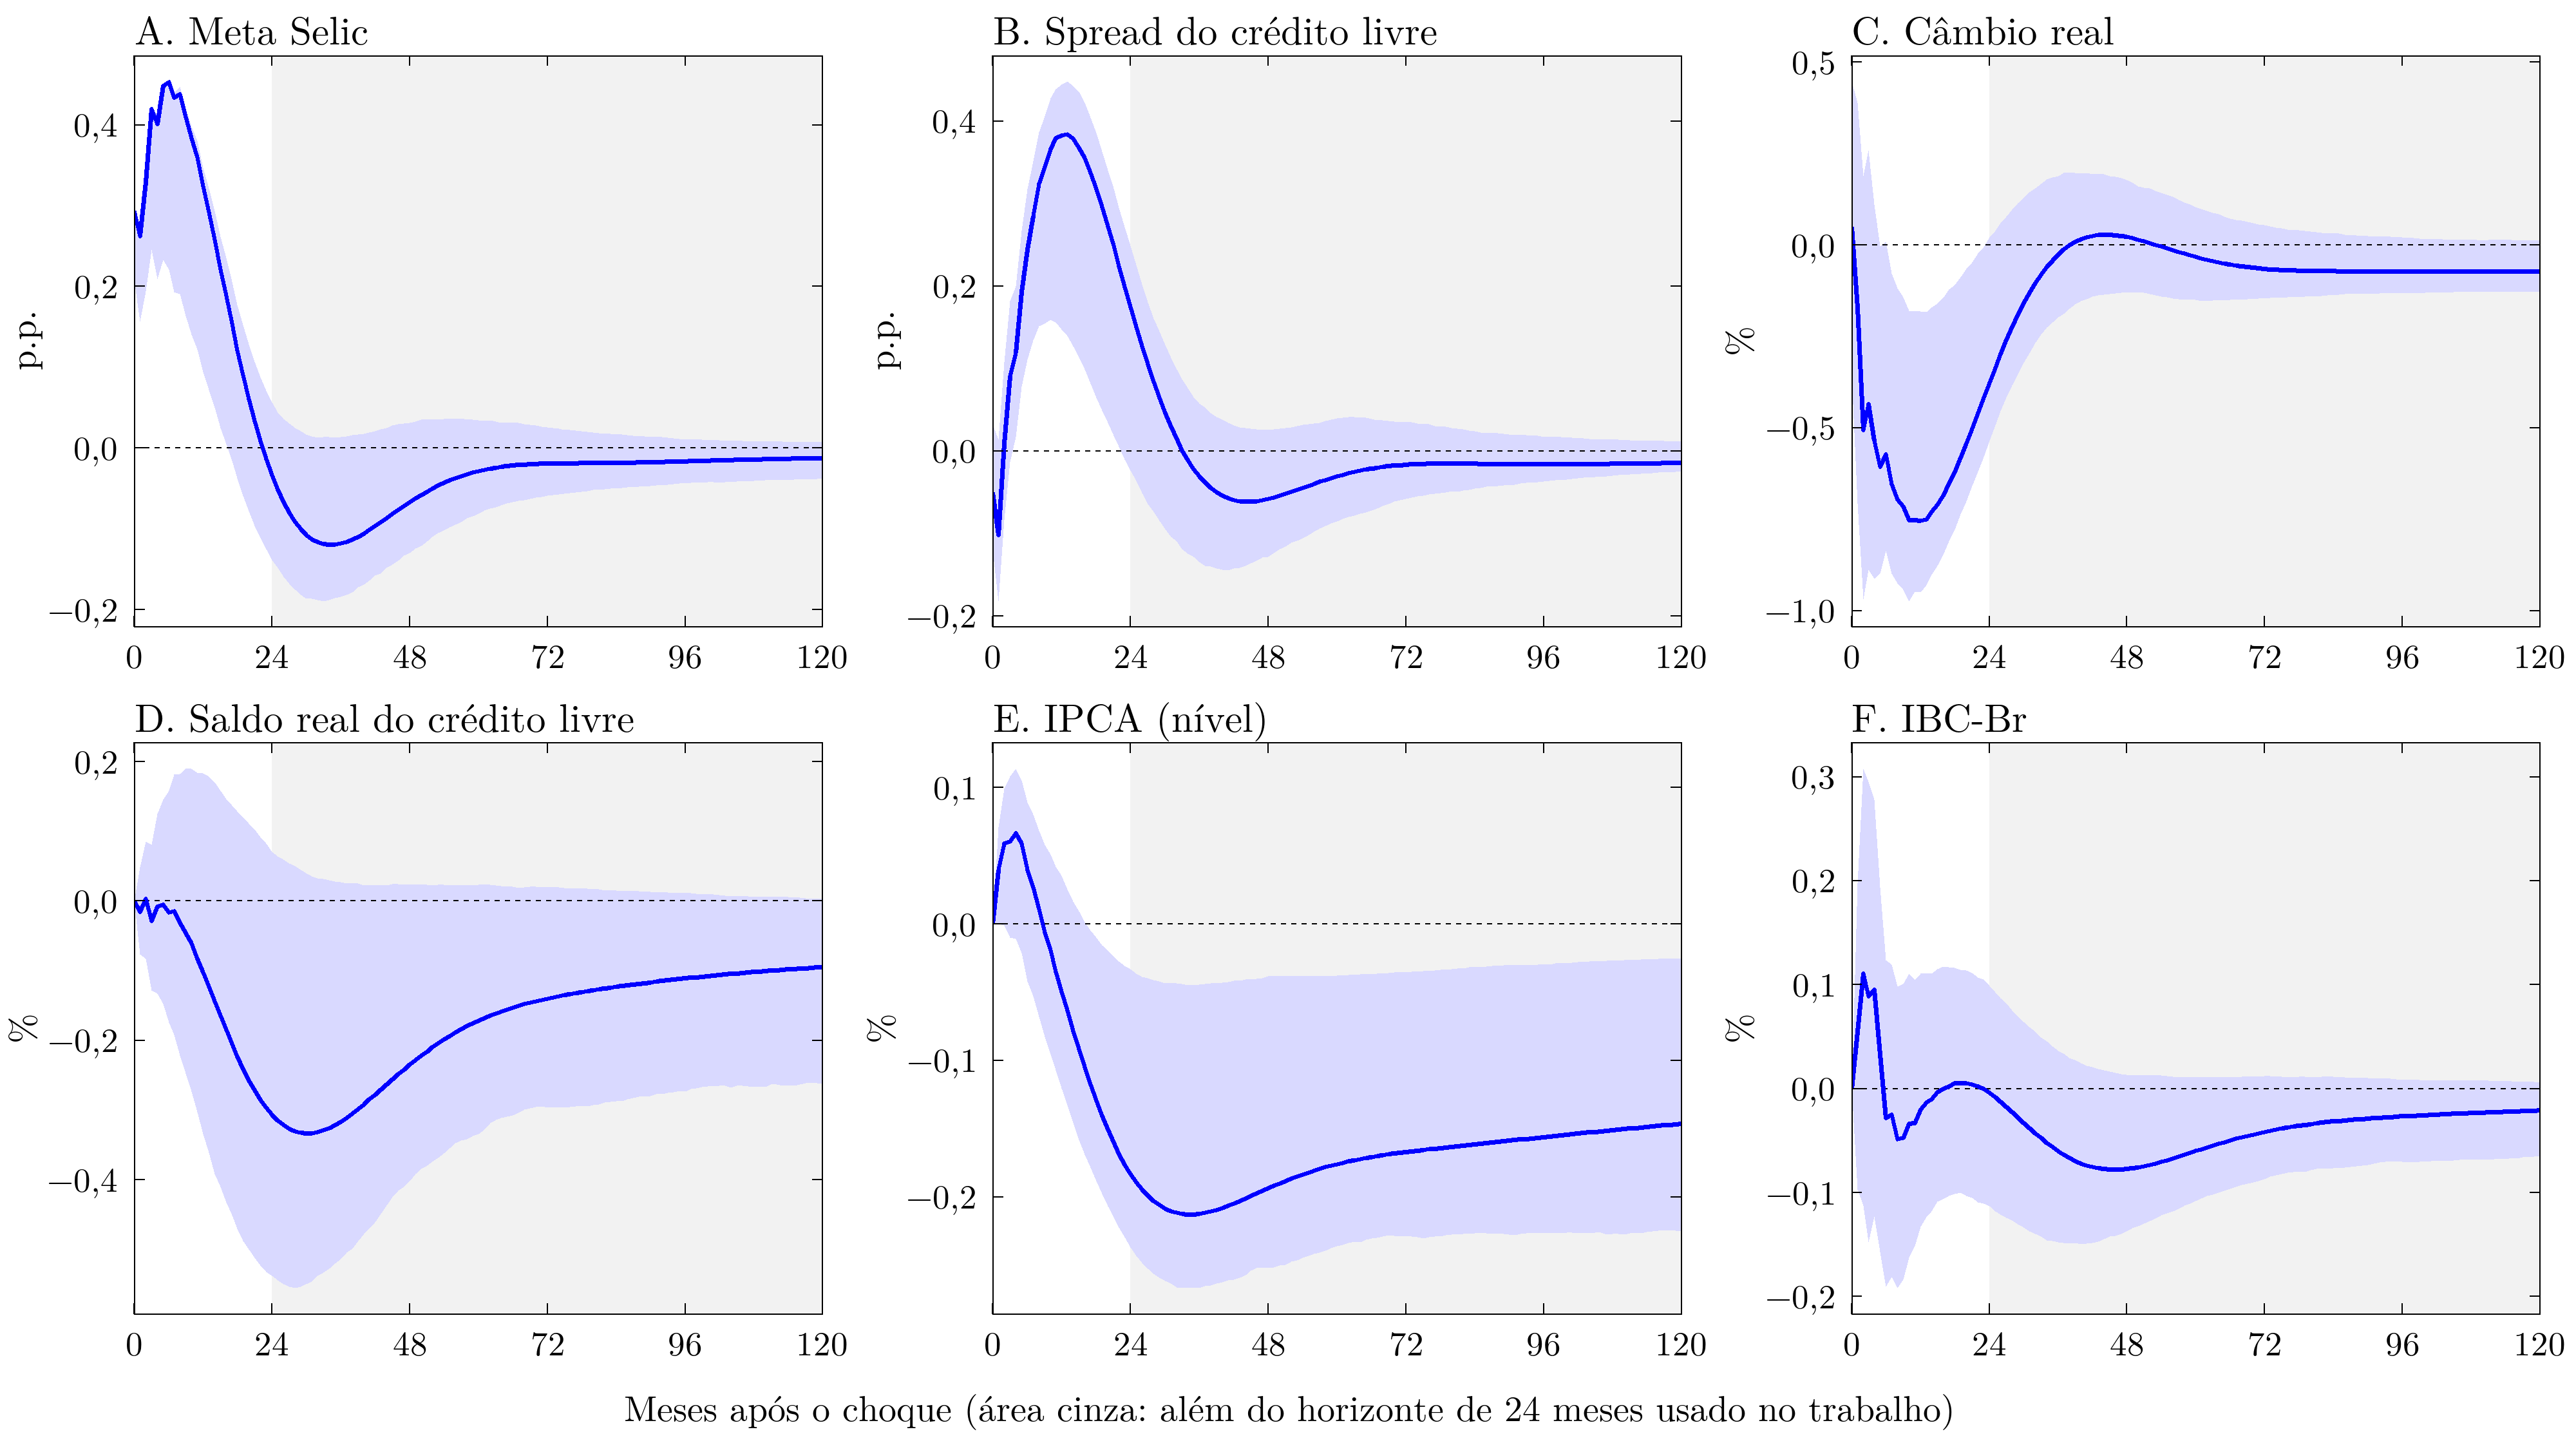
\includegraphics[width=0.66\textwidth]{slide_irf_120meses.png}
  \fonte{Choque de 1 d.p. na meta Selic. IC de 95\%, bootstrap com 5.000 réplicas.}
  \vspace{2pt}
  \raggedright\small
  Séries muito persistentes (maior raiz de \alert{0,998}): Selic, spread e câmbio perdem significância no segundo ano e voltam para perto de zero; o \alert{nível de preços} fica abaixo do inicial.\\[2pt]
  \voltar{resultado1}{Resultado 1}\indicereserva
\end{frame}

\begin{frame}[label=r-ordem]{Sensibilidade à ordenação das variáveis}
  \centering\small
  \begin{tabular}{@{}lcccccc@{}}
    \toprule
    & \multicolumn{2}{c}{Spread} & \multicolumn{2}{c}{Saldo real} & IBC-Br \\
    \cmidrule(lr){2-3}\cmidrule(lr){4-5}\cmidrule(l){6-6}
    Ordenação & 12 meses & Meses sig. & 24 meses & Meses sig. & Meses sig. \\
    \midrule
    Principal               & 0,38 & 4--22 & $-$0,31 & n.s. & 1--2 ($-$); 12--24 ($+$) \\
    Saldo depois da Selic   & 0,39 & 4--21 & $-$0,32 & n.s. & 1--2 ($-$); 12--24 ($+$) \\
    Selic em primeiro lugar & 0,39 & 4--21 & $-$0,31 & n.s. & 1--2 ($-$); 12--24 ($+$) \\
    Câmbio antes da Selic   & 0,38 & 4--21 & $-$0,29 & n.s. & 1--2 ($-$); 12--24 ($+$) \\
    Spread antes da Selic   & 0,37 & 3--21 & $-$0,29 & n.s. & 1--2 ($-$); 12--24 ($+$) \\
    \bottomrule
  \end{tabular}
  \fonte{Choque de 1 d.p. na meta (0,29 p.p. em todas). IBC-Br: resposta a choque no saldo. IC de 95\%, bootstrap com 5.000 réplicas.}
  \vspace{6pt}
  \raggedright
  A inovação da meta Selic tem correlação \alert{inferior a 0,1} com as das demais variáveis: sua posição na ordenação pouco altera o choque.\\[6pt]
  \voltar{modelo}{Modelo}\indicereserva
\end{frame}

\begin{frame}[label=r-testes]{Raiz unitária e cointegração}
  \begin{columns}[T]
    \begin{column}{0.56\textwidth}
      \centering\scriptsize
      \begin{tabular}{@{}lrrrr@{}}
        \toprule
        & \multicolumn{2}{c}{Nível} & \multicolumn{2}{c}{1ª diferença} \\
        \cmidrule(lr){2-3}\cmidrule(l){4-5}
        Série & ADF & KPSS & ADF & KPSS \\
        \midrule
        IBC-Br (log)       & $-$1,61   & 0,83*** & $-$9,61*** & 0,14 \\
        IPCA (log)         & $-$1,92   & 3,52*** & $-$5,40*** & 0,13 \\
        Saldo real (log)   & $-$3,61** & 2,21*** & $-$1,36    & 0,55** \\
        Meta Selic         & $-$3,09   & 0,37*   & $-$2,70*   & 0,27 \\
        Spread             & $-$3,18*  & 0,38*   & $-$2,70*   & 0,13 \\
        Câmbio real (log)  & $-$2,64   & 2,71*** & $-$8,27*** & 0,10 \\
        \bottomrule
      \end{tabular}
      \fonte{***, ** e *: rejeição a 1\%, 5\% e 10\%. H0: raiz unitária (ADF) e estacionariedade (KPSS).}
    \end{column}
    \begin{column}{0.42\textwidth}
      \centering\scriptsize
      \begin{tabular}{@{}ccccc@{}}
        \toprule
        & \multicolumn{2}{c}{Com dummies} & \multicolumn{2}{c}{Sem dummies} \\
        \cmidrule(lr){2-3}\cmidrule(l){4-5}
        Defas. & Traço & Máx. & Traço & Máx. \\
        \midrule
        2 & 5 & 5 & 3 & 3 \\
        3 & 5 & 5 & 3 & 2 \\
        4 & 5 & 3 & 3 & 1 \\
        5 & 5 & 5 & 2 & 1 \\
        6 & 5 & 3 & 2 & 1 \\
        \bottomrule
      \end{tabular}
      \fonte{Número de relações de cointegração (Johansen, 5\%).}
    \end{column}
  \end{columns}
  \vspace{8pt}
  \small
  Os testes não chegam a um quadro claro, e o número de relações varia de \alert{uma a cinco}: estimar em nível evita impor essas relações.\\[6pt]
  \voltar{modelo}{Modelo}\indicereserva
\end{frame}

\begin{frame}[label=r-defasagens]{Defasagens e autocorrelação dos resíduos}
  \centering\small
  \begin{tabular}{@{}ccccccccc@{}}
    \toprule
    & \multicolumn{6}{c}{Ljung-Box, por equação (p-valor)} & \multicolumn{2}{c}{Sistema} \\
    \cmidrule(lr){2-7}\cmidrule(l){8-9}
    Defas. & IBC-Br & IPCA & Saldo & Selic & Spread & Câmbio & LM & Raiz máx. \\
    \midrule
    2 & 0,50 & 0,68 & 0,28 & \alert{0,01} & 0,07 & 0,18 & 0,000 & 0,997 \\
    3 & 0,50 & 0,68 & 0,47 & \alert{0,02} & 0,58 & 0,54 & 0,000 & 0,998 \\
    \alert{4} & 0,75 & 0,81 & 0,44 & 0,78 & 0,37 & 0,47 & 0,000 & 0,998 \\
    5 & 0,99 & 0,58 & 0,37 & 0,81 & 0,58 & 0,59 & 0,038 & 0,997 \\
    6 & 0,95 & 0,72 & 0,23 & 0,92 & 0,66 & 0,48 & 0,000 & 0,997 \\
    \bottomrule
  \end{tabular}
  \fonte{Ljung-Box com 12 defasagens; LM de Edgerton-Shukur com 6 defasagens.}
  \vspace{6pt}
  \raggedright
  \begin{itemize}
    \item AIC e Hannan-Quinn indicam 2 defasagens, e Schwarz, 1; com menos de 4, a \alert{equação da Selic} mantém autocorrelação
    \item O teste conjunto ainda rejeita: por isso a verificação por projeções locais, com erros-padrão robustos
  \end{itemize}
  \voltar{modelo}{Modelo}\indicereserva
\end{frame}

\begin{frame}[label=r-choque]{O tamanho do choque}
  \begin{itemize}
    \item O choque é \alert{1 desvio-padrão} da inovação estrutural da meta Selic: \alert{0,29 p.p.} no mês do choque
    \item Como o modelo é linear, para uma alta de \alert{1 p.p.} basta multiplicar as respostas por cerca de \alert{3,4}
  \end{itemize}
  \vspace{6pt}
  \centering
  \begin{tabular}{@{}lcc@{}}
    \toprule
    Resposta & Choque de 0,29 p.p. & Choque de 1 p.p. \\
    \midrule
    Pico do spread (perto de 12 meses)     & 0,38 p.p. & $\approx$ 1,3 p.p. \\
    Saldo real do crédito livre (24 meses) & $-$0,31\% & $\approx -$1,1\% \\
    \bottomrule
  \end{tabular}\\[10pt]
  \raggedright
  \voltar{modelo}{Modelo}\indicereserva
\end{frame}

\begin{frame}[label=r-dummies]{Dummies do modelo}
  \begin{itemize}
    \item \alert{Onze dummies sazonais centradas}: o saldo e o spread não são dessazonalizados na fonte
    \item \alert{Dummies de eventos}: recessões de 2015 e 2016, greve dos caminhoneiros (mai.--jul./2018), período eleitoral de 2018, pandemia (mar.--dez./2020) e crise fiscal do fim de 2021
  \end{itemize}
  \vspace{4pt}
  \begin{block}{Sem as dummies de eventos}
    A alta do spread continua significativa entre o 4º e o 21º mês, com magnitude maior. O efeito do saldo sobre o IBC-Br deixa de ser significativo.
  \end{block}
  \vspace{4pt}
  \voltar{dados}{Dados}\indicereserva
\end{frame}

\begin{frame}[label=r-spread]{Definição do spread}
  \begin{block}{Spread médio das operações com recursos livres (BCB)}
    Taxa média de juros das \alert{novas operações} menos o \alert{custo de captação referencial médio}, calculado pelo próprio Banco Central
  \end{block}
  \vspace{4pt}
  \begin{itemize}
    \item \alert{Não} é a diferença em relação ao CDI ou à Selic
    \item Por isso, uma alta do spread após o choque significa que a taxa ao tomador sobe \alert{mais} que o custo de captação dos bancos
  \end{itemize}
  \vspace{4pt}
  \voltar{dados}{Dados}\indicereserva
\end{frame}

\begin{frame}[label=r-series]{Séries do modelo}
  \centering
  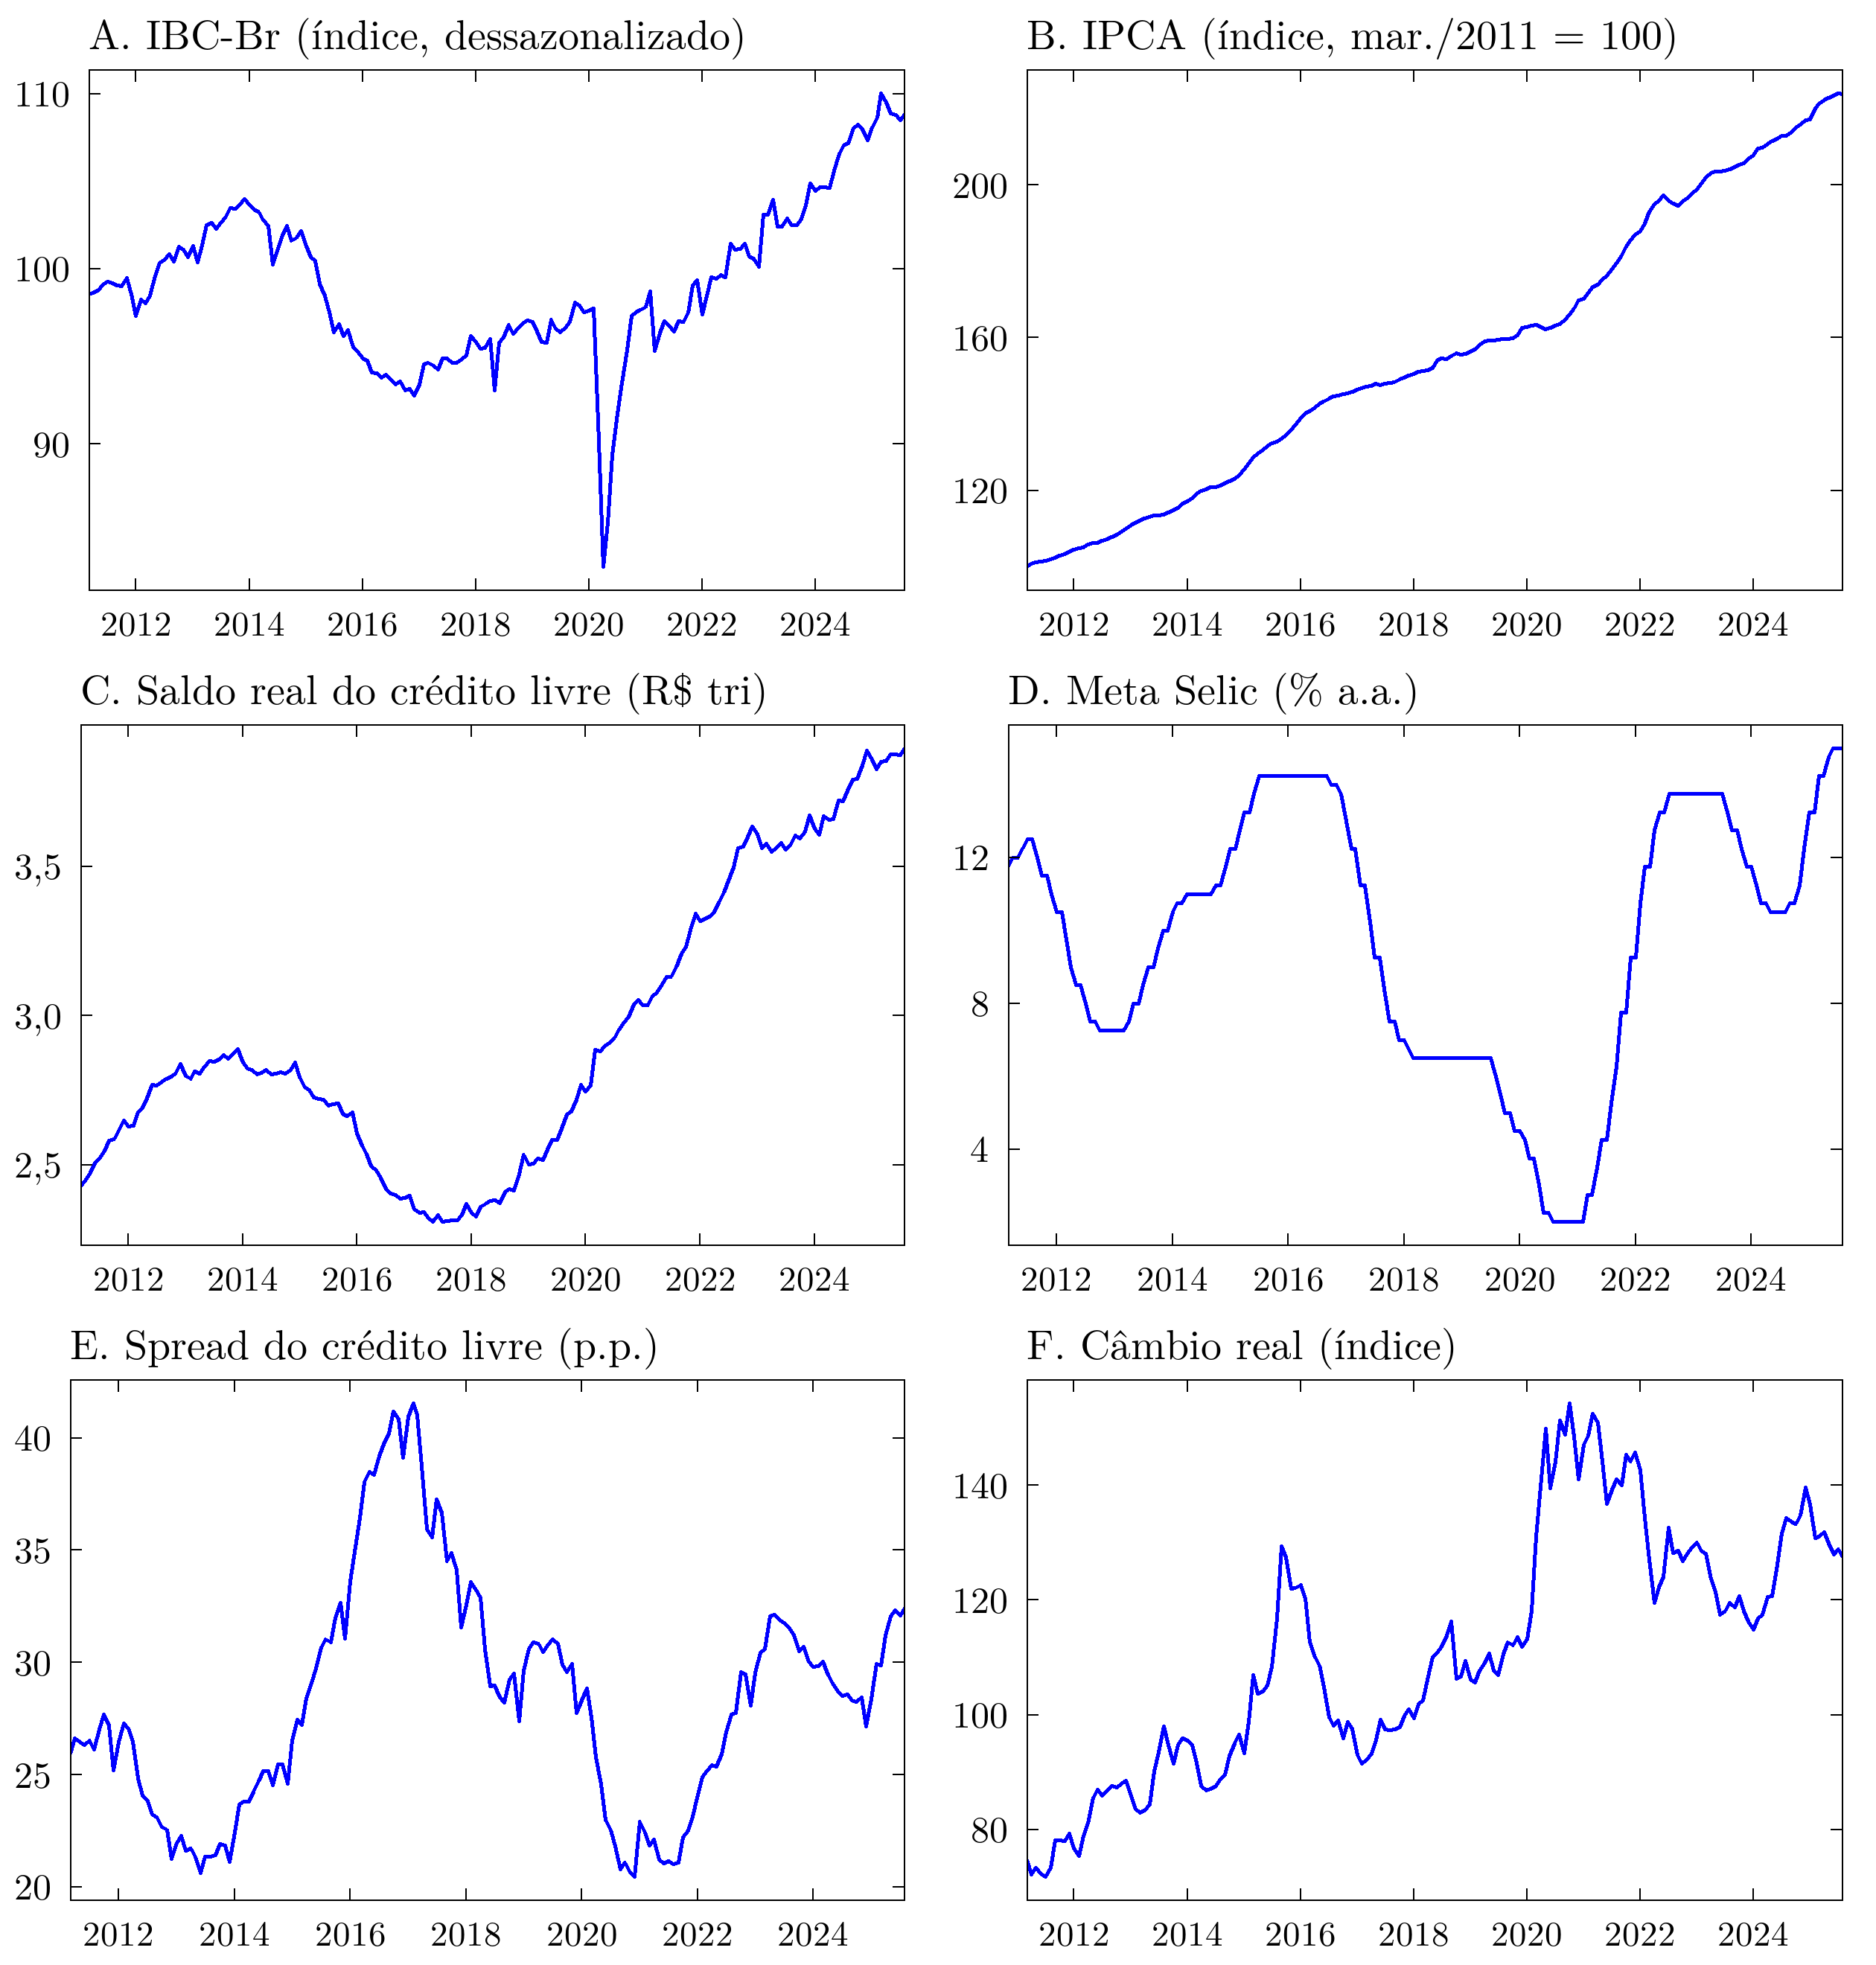
\includegraphics[height=0.78\textheight]{latex_fig06_series_modelo.png}\\
  \voltar{dados}{Dados}\indicereserva
\end{frame}

\begin{frame}[label=r-fevd]{Decomposição da variância do erro de previsão (\%)}
  \centering\small
  \begin{tabular}{@{}lrrrrrr@{}}
    \toprule
    & \multicolumn{6}{c}{Choque em} \\
    \cmidrule(l){2-7}
    Variável & IBC-Br & IPCA & Saldo real & Meta Selic & Spread & Câmbio \\
    \midrule
    \multicolumn{7}{@{}l}{\textit{Horizonte de 12 meses}} \\
    IBC-Br     & 76,8 & 3,7  & 10,7 & 0,9  & 4,3  & 3,5  \\
    Saldo real & 0,3  & 2,0  & 62,6 & 0,2  & 1,4  & 33,5 \\
    Spread     & 11,5 & 0,2  & 18,6 & 28,9 & 27,9 & 12,8 \\
    IPCA       & 2,5  & 76,1 & 7,5  & 2,5  & 3,2  & 8,2  \\
    \multicolumn{7}{@{}l}{\textit{Horizonte de 24 meses}} \\
    IBC-Br     & 64,0 & 3,2  & \alert{15,4} & \alert{0,7} & 4,1 & 12,6 \\
    Saldo real & 0,2  & 1,7  & 55,9 & 2,6  & 2,2  & 37,3 \\
    Spread     & 5,7  & 0,3  & 22,7 & \alert{37,5} & 18,4 & 15,5 \\
    IPCA       & 1,5  & 49,4 & 30,4 & 10,5 & 1,7  & 6,5  \\
    \bottomrule
  \end{tabular}\\[8pt]
  \raggedright
  \voltar{fevd}{Decomposição da variância}\indicereserva
\end{frame}

\begin{frame}[label=r-compl]{Respostas complementares}
  \begin{columns}[c]
    \begin{column}{0.52\textwidth}
      \centering
      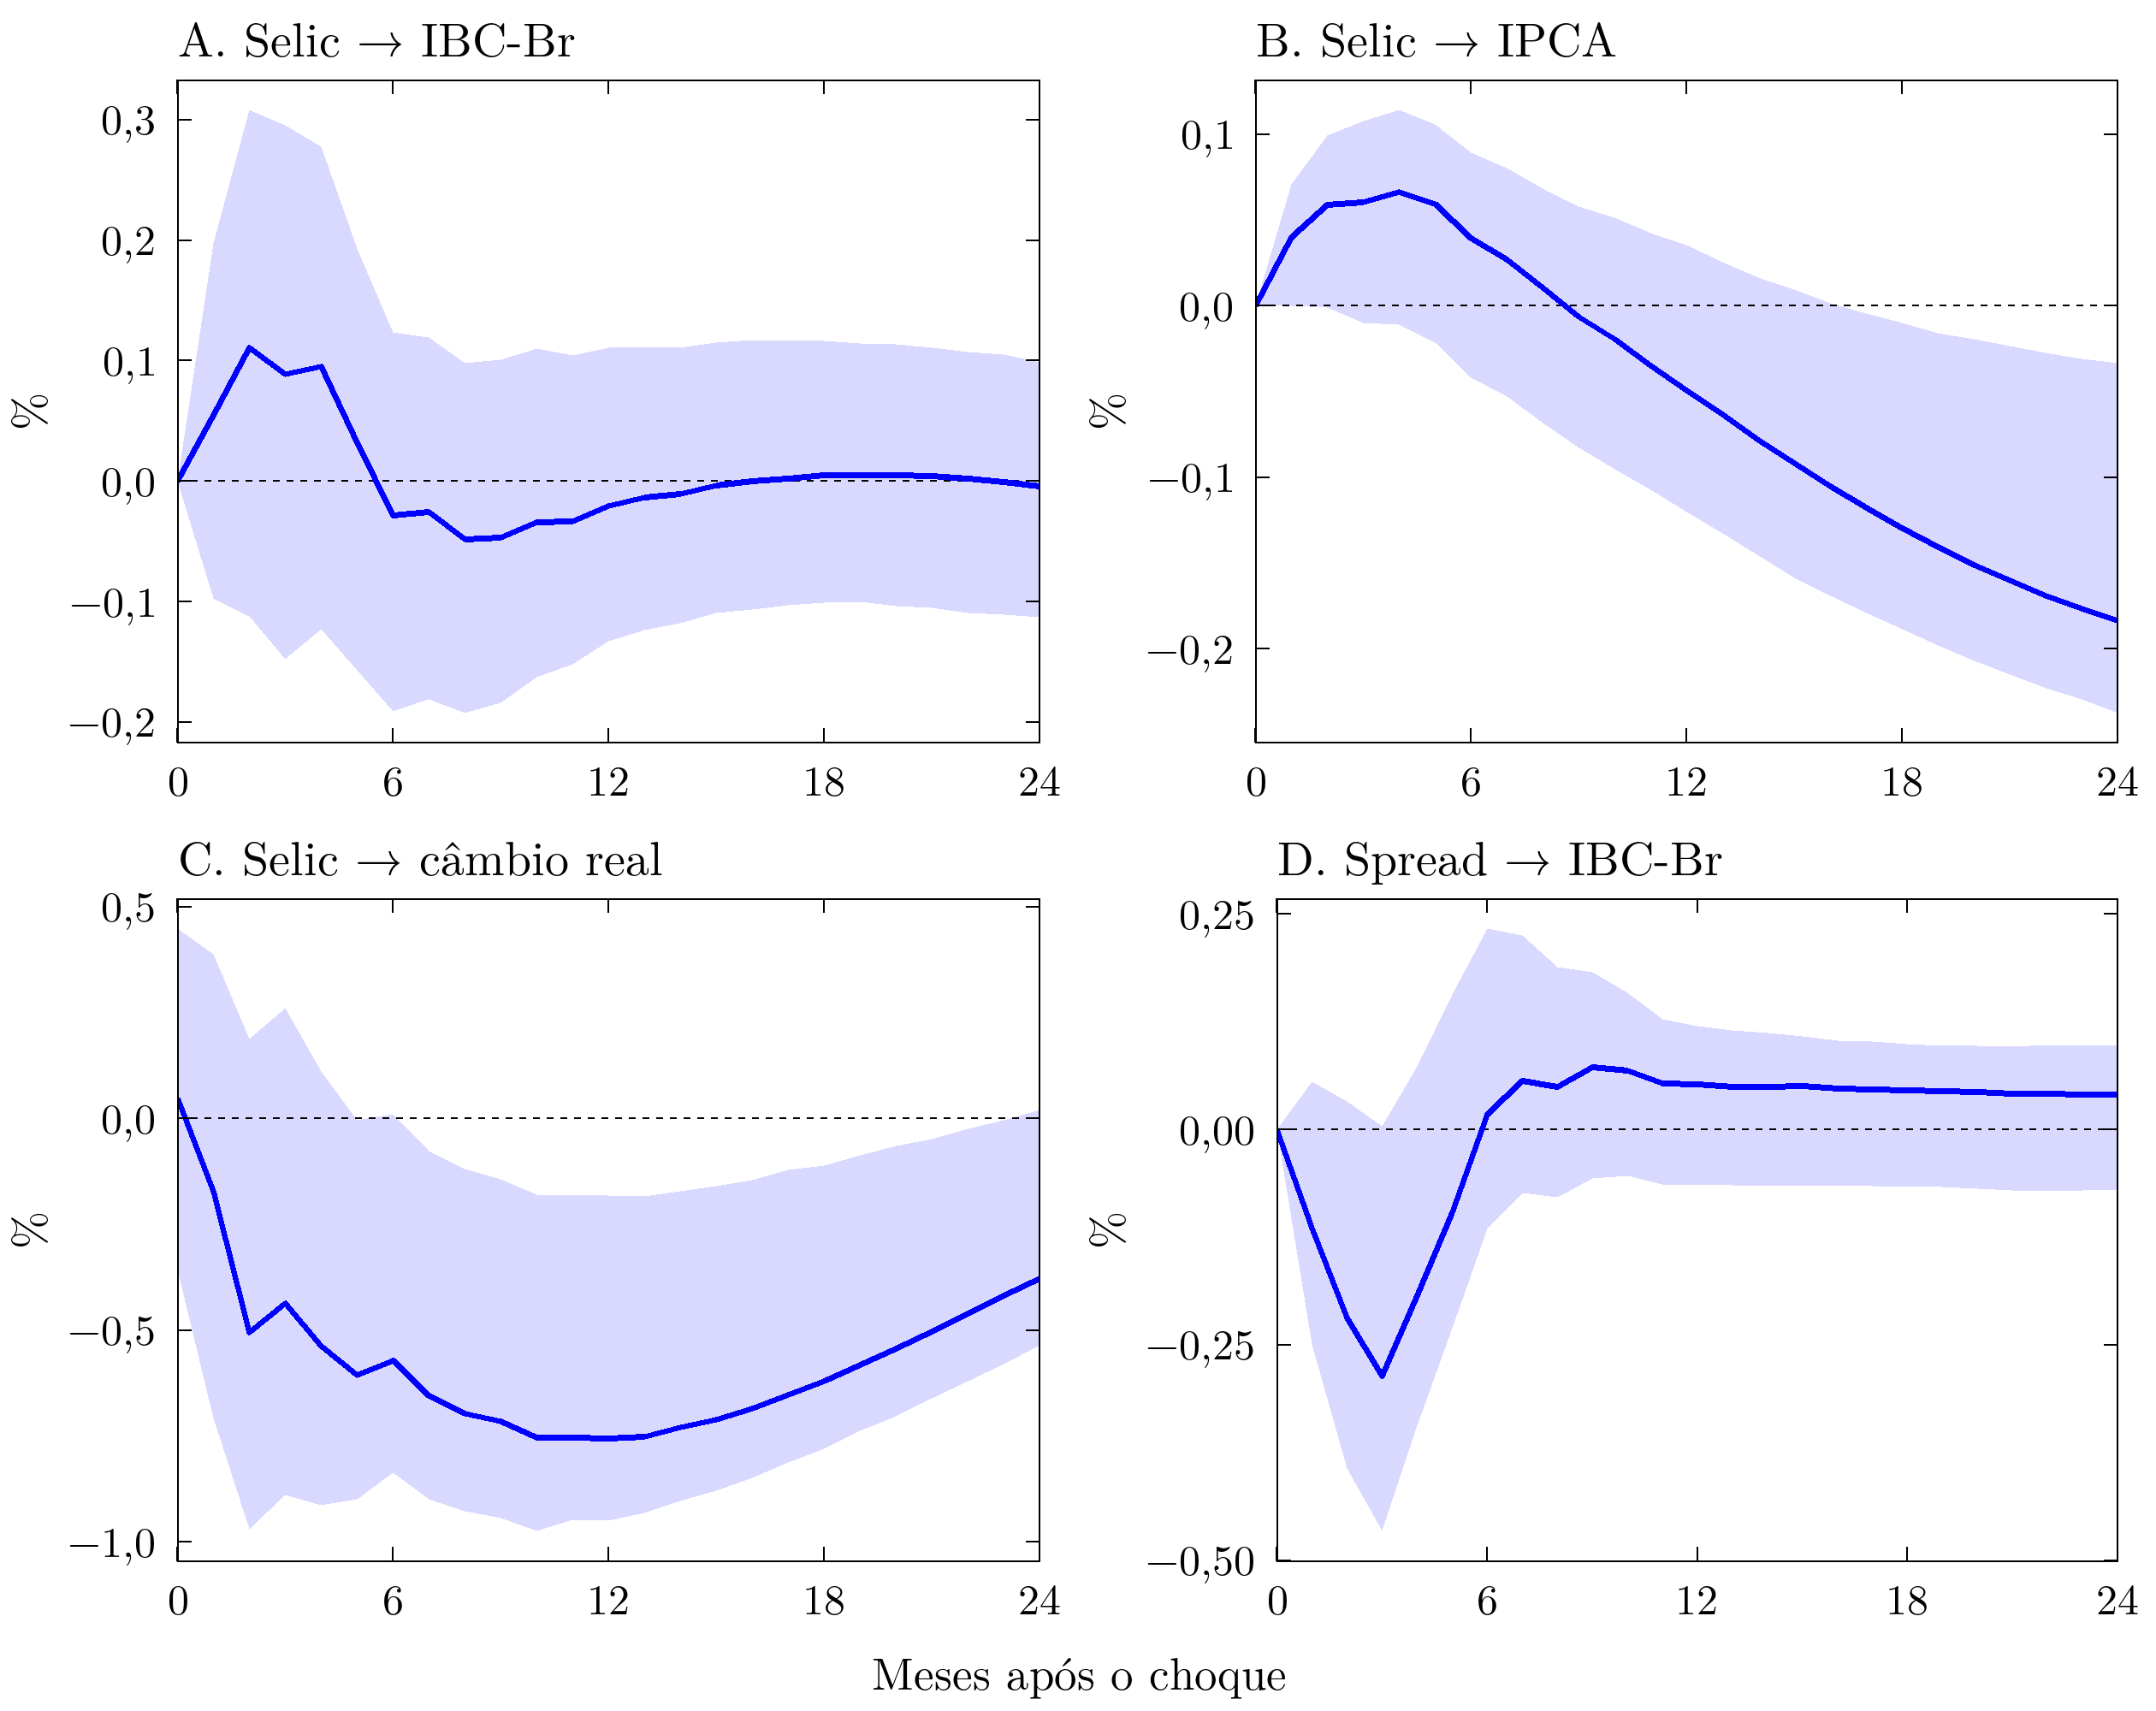
\includegraphics[width=\linewidth]{latex_fig11_complementares.png}
    \end{column}
    \begin{column}{0.46\textwidth}
      \small
      \begin{itemize}
        \item IBC-Br: resposta à Selic não significativa em nenhum horizonte
        \item IPCA: \alert{cai no segundo ano} após o choque
        \item Câmbio real: \alert{aprecia} após o aperto
        \item Spread $\rightarrow$ IBC-Br: queda de curto prazo
      \end{itemize}
      \fonte{Choque de 1 d.p. IC de 95\%, bootstrap com 5.000 réplicas.}
      \vspace{4pt}
      \voltar{fevd}{Decomposição da variância}\\[3pt]
      \hyperlink{reservas}{\beamerskipbutton{Índice da reserva}}
    \end{column}
  \end{columns}
\end{frame}

\begin{frame}[label=r-direcionado]{Robustez: crédito livre e direcionado}
  \begin{itemize}
    \item \alert{Saldo direcionado}: série 20593 do SGS, deflacionada pelo IPCA, no mesmo VAR do crédito livre
    \item \alert{Projeções locais com os dois saldos}: só o livre cai de forma significativa, entre o 10º e o 19º mês
    \item Com o direcionado no lugar do livre, sua resposta à Selic segue \alert{não significativa} com seis defasagens, sem as dummies de eventos ou em proporção do PIB
    \item \alert{Crédito total}: modelo em \% do PIB com meta Selic, IBC-Br, IPCA e câmbio, de jan./2003 a ago./2025 e cinco defasagens; o spread fica de fora porque a série começa em 2011
  \end{itemize}
  \vspace{6pt}
  \voltar{segmentos}{Teste da segmentação}\indicereserva
\end{frame}

\begin{frame}[label=r-taxas]{Taxas médias de juros por segmento}
  \centering
  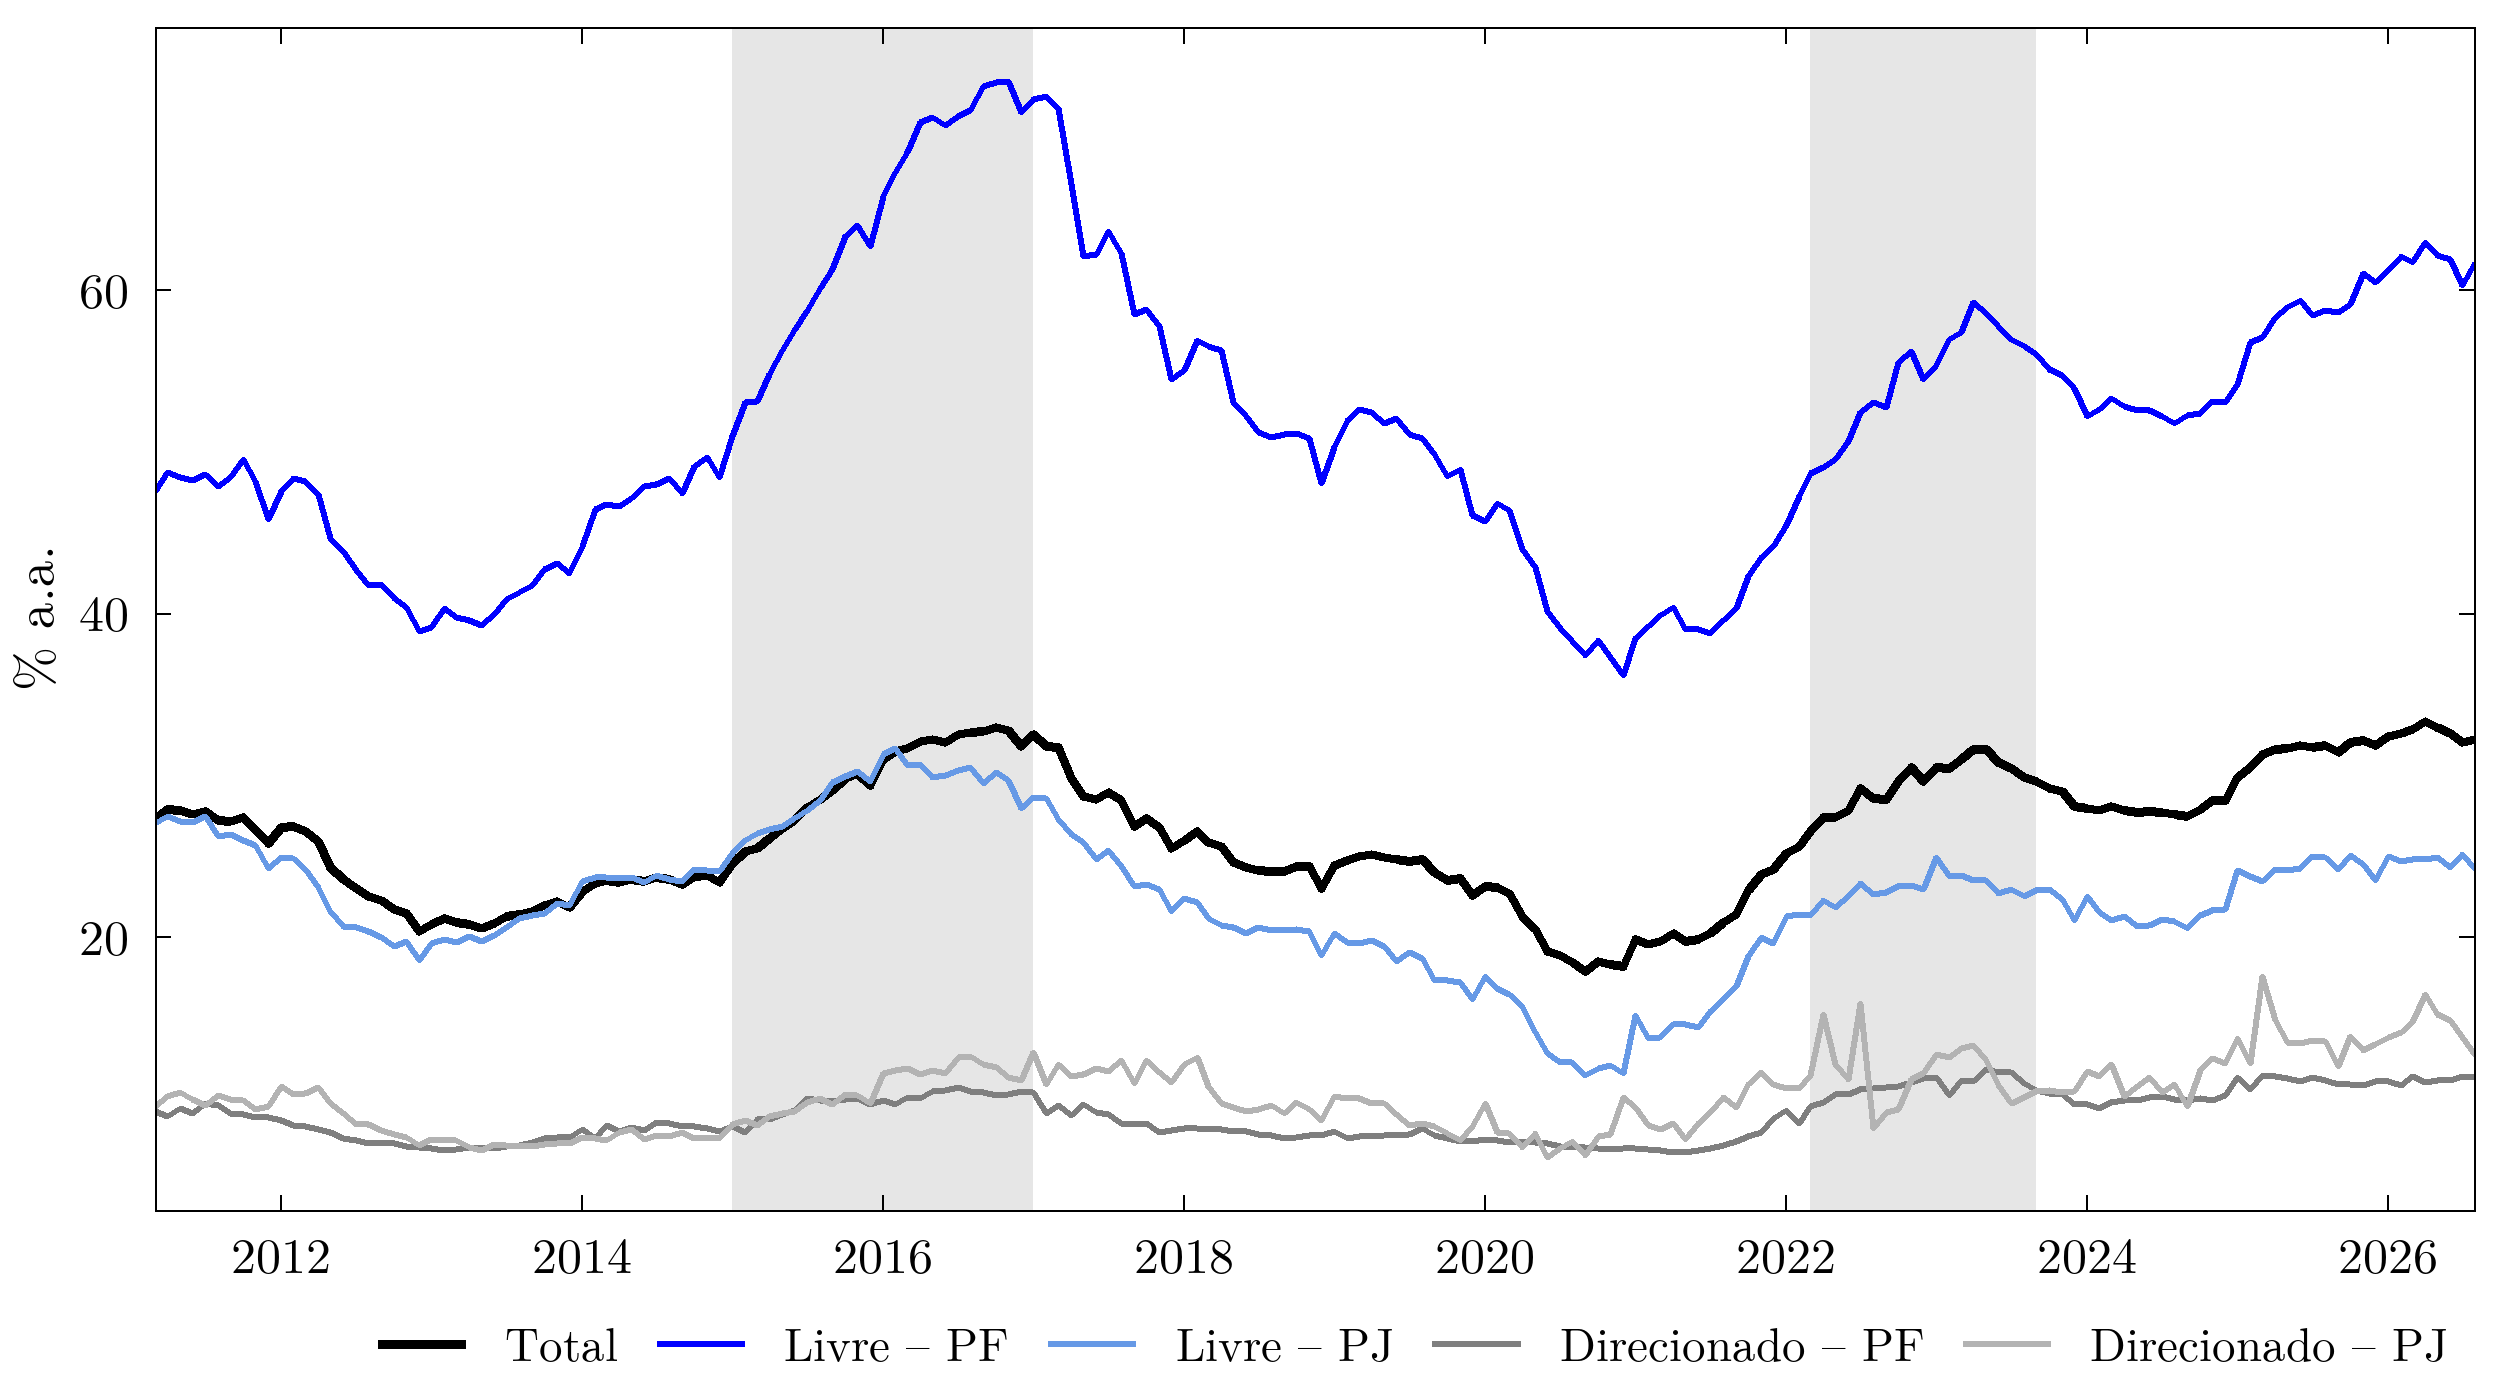
\includegraphics[width=0.68\textwidth]{latex_fig05_taxas_segmento.png}
  \fonte{Taxa média de juros do SFN por segmento (\% a.a.). Áreas sombreadas: ciclos de aperto monetário. Fonte: BCB (SGS).}
  \vspace{4pt}
  \raggedright
  \voltar{taxas}{Preço do crédito}\indicereserva
\end{frame}

\begin{frame}[label=r-concessoes]{Concessões de crédito direcionado}
  \centering
  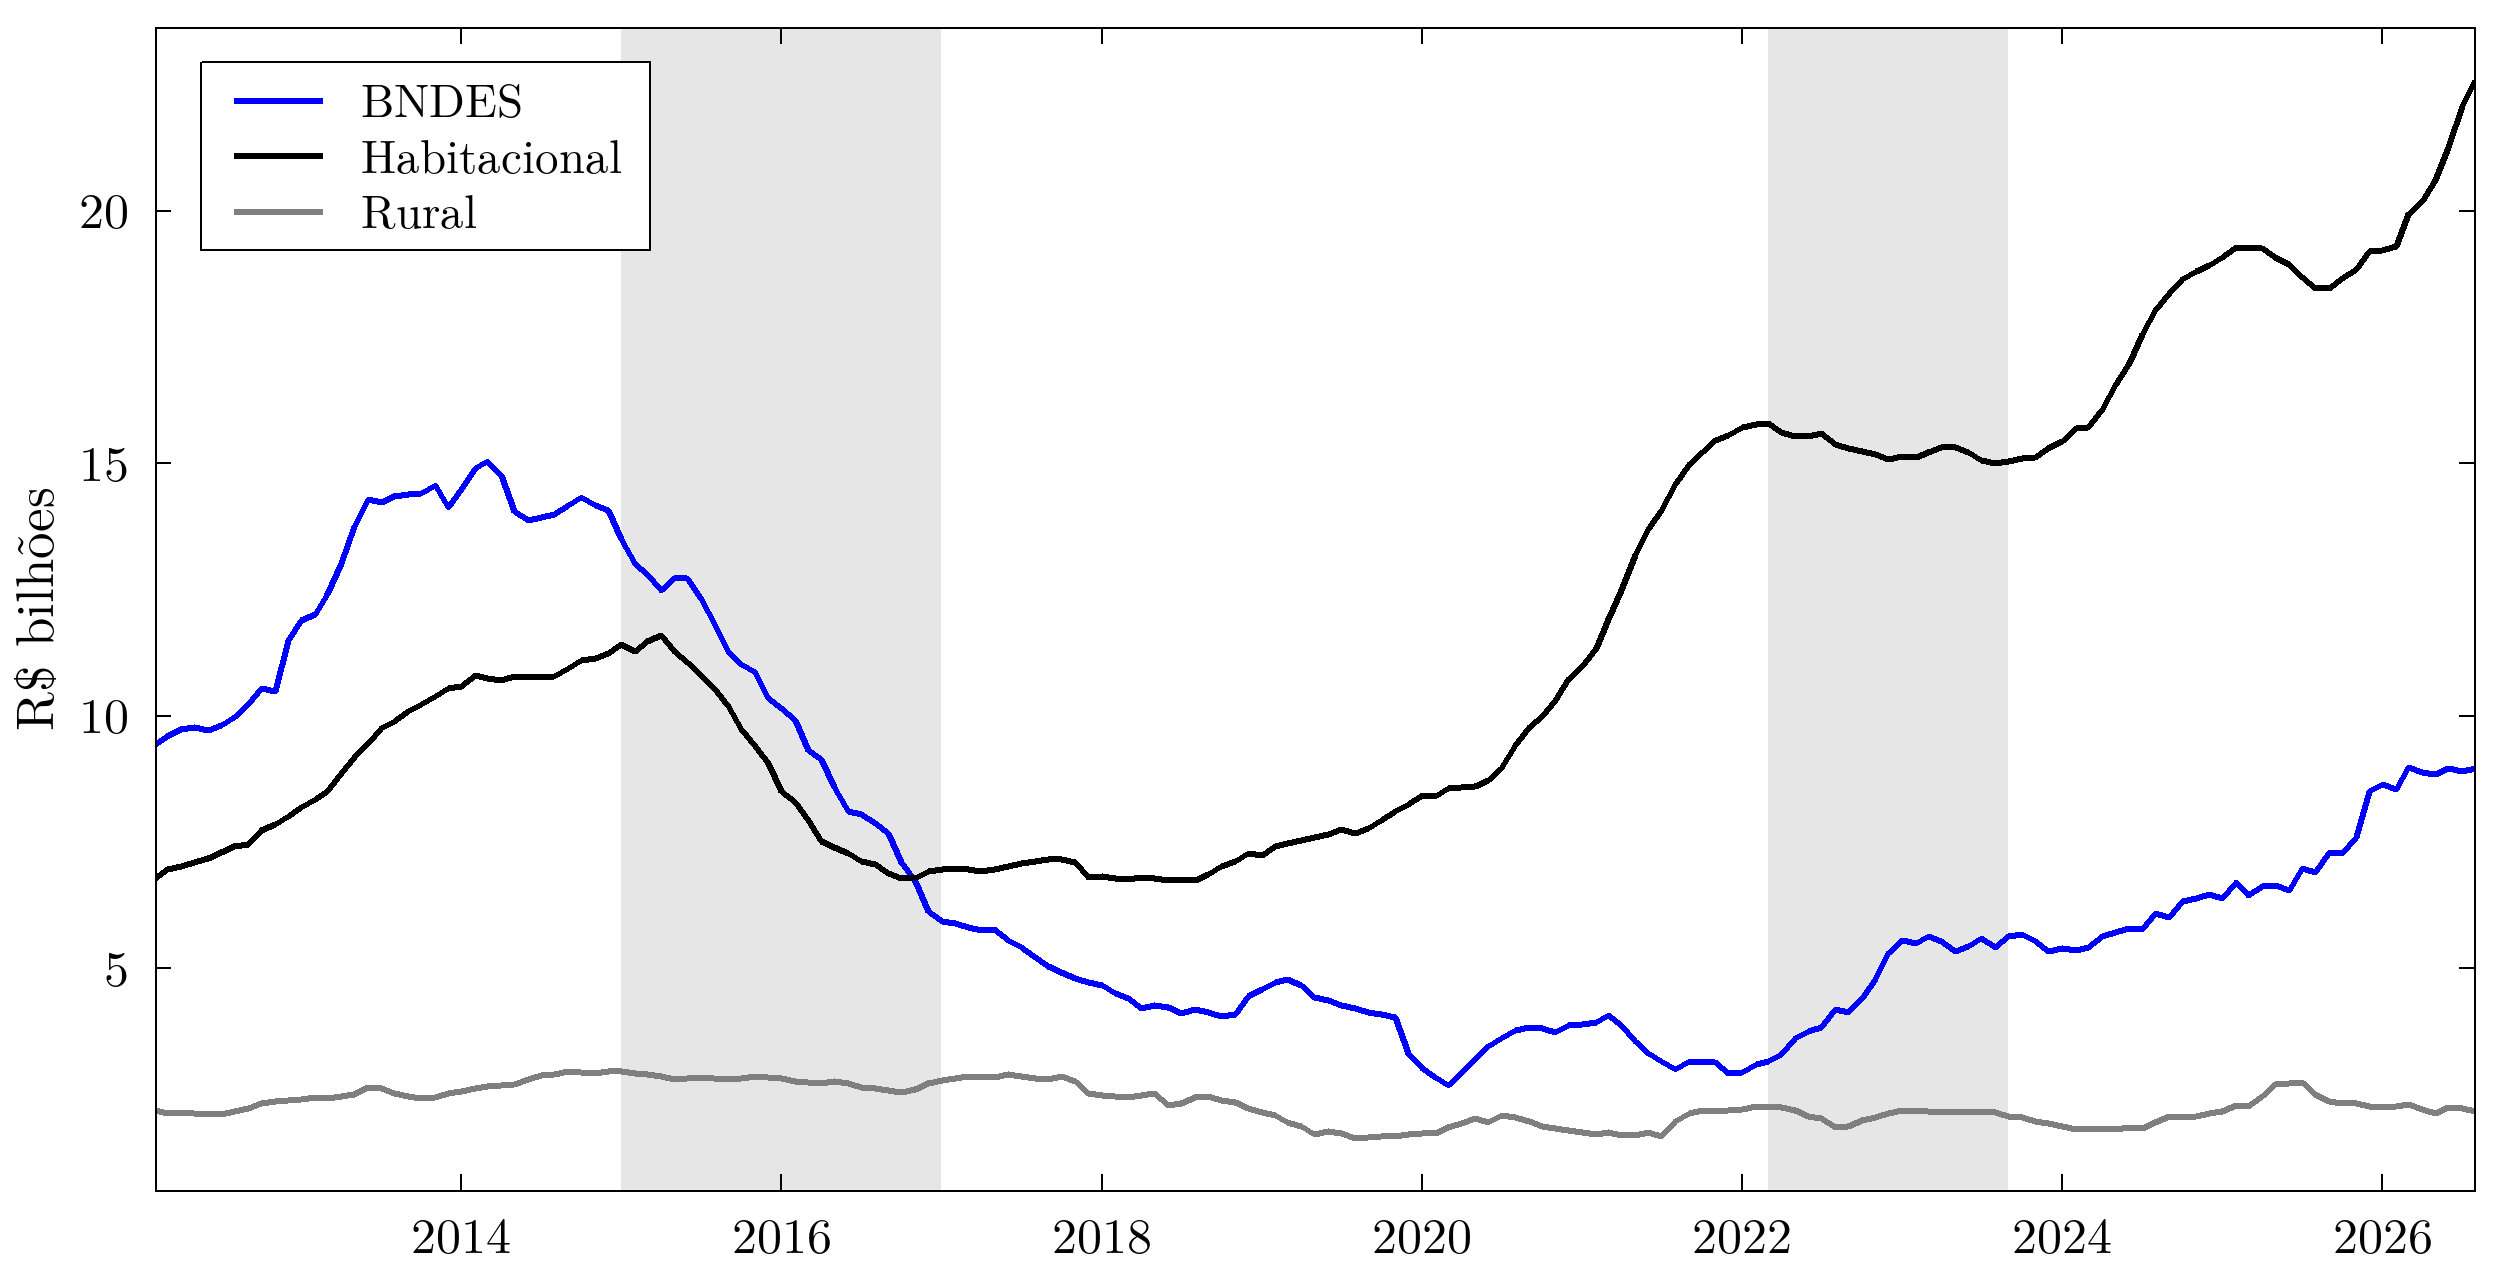
\includegraphics[width=0.70\textwidth]{latex_fig04_concessoes.png}
  \fonte{Concessões por modalidade (R\$ bilhões), médias móveis de 12 meses. Áreas sombreadas: ciclos de aperto monetário. Fonte: BCB (SGS).}
  \vspace{4pt}
  \raggedright
  \voltar{segmentacao}{Segmentação}\indicereserva
\end{frame}

\end{document}
